\documentclass{beamer}
\usepackage{graphicx}

\usepackage{url}

\usepackage{amsmath}
\usepackage{amssymb}
\usepackage{xkeyval}

\usepackage{../macros/mytikz}
\usepackage{listings}
\lstset{mathescape}

\usepgflibrary{shapes}
\usepackage{stmaryrd}

\usepackage{../macros/basics}
\usepackage{../macros/basics-slides}
%\usepackage{../macros/mmt_listings}
\usepackage{../macros/twelf-math}

\usepackage{../macros}
\usepackage{macros}


\newcommand{\lf}{\mathit{LF}}
\newcommand{\kity}{\mathit{type}}


\renewcommand{\emph}[1]{\alert{#1}}

%\setbeamertemplate{headline}{\small\hfill\insertsection \hfill\hbox{}}

\begin{document}

\title{Knowledge Representation and Processing}
\author{Florian Rabe (for a course given with Michael Kohlhase)}
\institute{Computer Science, University Erlangen-N\"urnberg, Germany}
\date{Summer 2021}
\begin{frame}
    \titlepage
\end{frame}

\part{Introduction}

\section{Administrative Information}

\begin{frame}\frametitle{Format}
\begin{blockitems}{Zoom}
\item lectures and exercises via zoom
\item interaction strongly encouraged
 \lec{We don't want to lecture ---}
 \lec{we want to have a conversation during which you learn}
\item mae use of zoom
 \begin{itemize}
 \item use reactions to say yes no, ask for break etc.
 \item feel free to annotate my slides
 \item talk in the chat
 \end{itemize}
\end{blockitems}

\begin{blockitems}{Recordings}
\item maybe prerecorded video lectures or recorded zoom meeting
\item to be decided along the way
\end{blockitems}
\end{frame}


\begin{frame}\frametitle{Background}
\begin{blockitems}{Instructors}
\item Prof. Dr. Michael Kohlhase \lec{Professor of Knowledge Representation and Processing}
\item PD Dr. Florian Rabe \lec{same research group}
\end{blockitems}

\begin{blockitems}{Course}
\item This course is given for the second time
\item First time was a little bit of an experiment
  \lec{polishing and revising the materials this year}
\item To become signature course of our research group \lec{same name!}
\end{blockitems}
\end{frame}

\begin{frame}\frametitle{Prerequisites}
\begin{blockitems}{Required}
\item basic knowledge about formal languages, context-free grammars
 \lec{but we'll do a quick revision here}
\end{blockitems}

\begin{blockitems}{Helpful}
\item Algorithms and Data Structures
 \lec{mostly as a contrast to this lecture}
\item Basic logic
 \lec{we'll revise it slightly differently here}
\item all other courses
 \lec{as examples of how knowledge pervades all of CS}
\end{blockitems}

\begin{blockitems}{General}
\item Curiosity \lec{this course is a bit unusual}
\item Interest in big picture \lec{this course touches on lots of things from all over CS}
\end{blockitems}
\end{frame}

\begin{frame}\frametitle{Examination and Grading}
\begin{blockitems}{Suggestion}
\item grade determined by single exam
\item oral, 30 minutes
\item exercises indirectly graded through conversation during exam
\end{blockitems}

\begin{blockitems}{Exam-relevant}
\item anything mentioned in notes
\item anything discussed in lectures
\item anything done in exercises
\end{blockitems}
\lec{neither is a superset of the other!}
\end{frame}

\begin{frame}\frametitle{Materials and Exam-Relevance}
\begin{blockitems}{Textbook}
\item does not exist
\item normal for research-near specialization courses
\end{blockitems}

\begin{blockitems}{Notes}
\item textbook-style but not as comprehensive
\item developed along the way
\end{blockitems}

\begin{blockitems}{Slides}
\item not comprehensive
\item used as visual aid, conversation starters
\end{blockitems}
\end{frame}

\begin{frame}\frametitle{Communication}
\begin{blockitems}{Open for questions}
\item open door policy in our offices
  \glec{if the lockdown ever ends}
\item always room for questions during lectures
\item for personal questions, contact me during/after lecture or by email
\item forum at \url{https://fsi.cs.fau.de/forum/154-Wissensrepraesentation-und-Verarbeitung}
\end{blockitems}

\begin{blockitems}{Materials}
\item official notes and slides as pdf: \url{https://kwarc.info/teaching/WuV/}
 \lec{will be updated from time to time}
\item watch me prepare the materials: \url{https://github.com/florian-rabe/Teaching/tree/master/WuV}
 \lec{pull requests and issues welcome}
\end{blockitems}
\end{frame}

\begin{frame}\frametitle{Exercises}
\begin{blockitems}{Learning Goals}
\item Get acquainted with state of the art of practice
\item Try out real tools
\end{blockitems}

\begin{blockitems}{Homeworks}
\item one major project as running example
\item homeworks building on each other
\end{blockitems}
\lec{build one large knowledge-based system}
\lec{details on later slides}
\end{frame}

\section{Overview and Essential Concepts}

\begin{frame}\frametitle{Representation and Processing}
Common pairs of concepts:
\begin{center}
\begin{tabular}{l|l}
Representation & Processing \\
\hline
Static & Dynamic \\
Situation & Change \\
Be & Become \\
Data Structures & Algorithms \\
Set & Function \\
State & Transition \\
Space & Time
\end{tabular}
\end{center}
\end{frame}

\begin{frame}\frametitle{Data and Knowledge}
$2\times 2$ key concepts
\begin{center}
\begin{tabular}{l|l}
Syntax & Data \\
\hline
Semantics & Knowledge
\end{tabular}
\end{center}

\begin{itemize}
\item Data: any object that can be stored in a computer\\
 Example: $((49.5739143, 11.0264941), "2020-04-21T16:15:00CEST")$
\item Syntax: a system of rules that describes which data is \textbf{well-formed}\\
 Example: ``a pair of (a pair of two IEEE double precision floating point numbers) and a string encoding of a time stamp''
\item Semantics: system of rules that determines the meaning of well-formed data
\item Knowledge: combination of some data with its syntax and semantics
\end{itemize}
\end{frame}

\begin{frame}\frametitle{Knowledge is Elusive}
Representation of key concepts 
\begin{itemize}
 \item Data: using primitive objects
  \lec{implemented as bits, bytes, strings, records, arrays, \ldots}
 \item Syntax: (context-free) grammars, (context-sensitive) type systems
  \lec{implemeted as inductive data structures}
 \item Semantics: functions for evaluation, interpretation, of well-formed data
  \lec{implemented as recursive algorithms on the syntax}
 \item Knowledge: elusive
  \lec{emerges from applying and interacting with the semantics}
\end{itemize}
\end{frame}

\begin{frame}\frametitle{Semantics as Translation}
\begin{itemize}
\item Knowledge can be captured by a higher layer of syntax
\item Then semantics is translation into syntax
\end{itemize}

\begin{center}
\begin{tabular}{l|l|l}
Data syntax & Semantics function & Knowledge syntax \\
\hline
SPARQL query & evaluation & result set \\
SQL query & evaluation & result table \\
program & compiler & binary code \\
program expression & interpreter & result value \\ 
logical formula & interpretation in a model & mathematical object \\
HTML document & rendering & graphics context
\end{tabular}
\end{center}
\end{frame}

\begin{frame}\frametitle{Heterogeneity of Data and Knowledge}
\begin{itemize}
\item Capturing knowledge is difficult
\item Many different approaches to semantics
 \begin{itemize}
  \item fundamental formal and methodological differences
  \item often captured in different fields, conferences, courses, languages, tools
 \end{itemize}
\item Data formats equally heterogeneous
 \begin{itemize}
 \item ontologies
 \item programs
 \item logical proofs
 \item databases
 \item documents
 \end{itemize}
\end{itemize}
\end{frame}

\begin{frame}\frametitle{Challenges of Heterogeneity}
\begin{blockitems}{Challenges}
\item collaboration across communities
\item translation across languages
\item conversion between data formats
\item interoperability across tools
\end{blockitems}

\begin{blockitems}{Sources of problems}
\item interoperability across formats/tools major source of
 \begin{itemize}
 \item complexity
 \item bugs
 \end{itemize}
\item friction in project team due to differing preferences, expertise
\item difficult choice between languages/tools with competing advantages
\begin{itemize}
 \item reverting choices difficult, costly
 \item maintaining legacy choices increases complexity
\end{itemize}
\end{blockitems}
\end{frame}

\begin{frame}\frametitle{Aspects of Knowledge}
\begin{itemize}
\item Tetrapod model of knowledge
  \lec{active research by our group}
\item classifies approaches to knowledge into five aspects
\end{itemize}

\begin{center}
\begin{tabular}{lll}
Aspect & KRLs (examples) & KPTs (examples) \\
\hline
ontologization & ontology languages (OWL), description logics (ALC) & reasoners, SPARQL engines (Virtuoso) \\
concretization & relational databases (SQL, JSON) & databases (MySQL, MongoDb) \\
computation & programming languages (C) & interpreters, compilers (gcc) \\
deduction & logics (HOL) & theorem provers (Isabelle) \\
narration & document languages (HTML, LaTeX) & editors, viewers
\end{tabular}
\end{center}
\end{frame}

\begin{frame}\frametitle{Relations between the Aspects}
Ontology is distinguished: capture the knowledge that the other four aspects share

\begin{center}
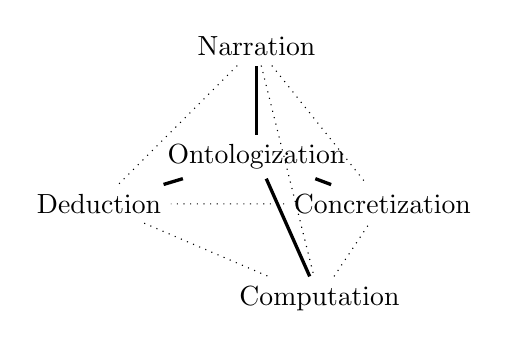
\begin{tikzpicture}[scale=4]
  \node (center) at (0,.15) {Ontologization};
  \node (left) at (.2,-.3) {Computation};
  \node (right) at (.4,0) {Concretization};
  \node (back) at (-.5,0) {Deduction};
  \node (up) at (0,.5) {Narration};

  \draw[very thick] (center) -- (left);
  \draw[very thick] (center) -- (right);
  \draw[very thick] (center) -- (back);
  \draw[very thick] (center) -- (up);
  \draw[dotted] (left) -- (right) -- (back) -- (left);
  \draw[dotted] (up) -- (left);
  \draw[dotted] (up) -- (right);
  \draw[dotted] (up) -- (back);
\end{tikzpicture}
\end{center}
\end{frame}

\begin{frame}\frametitle{Complementary Advantages of the Aspects}
\begin{center}
\footnotesize
\begin{tabular}{|l|llp{2.1cm}l|}\hline
Aspect & objects & \multicolumn{3}{c|}{characteristic} \\
       &         & advantage & joint advantage of the other aspects & application \\\hline
ded. & formal proofs & correctness & ease of use & verification \\
comp. & programs & efficiency & well-definedness & execution\\
concr. & concrete objects & tangibility & abstraction & storage/retrieval\\
narr. & texts & flexibility & formal semantics & human understanding\\\hline
\end{tabular}
\medskip

\begin{tabular}{|l|l|}\hline
Aspect pair & characteristic advantage \\\hline
ded./comp.  & rich meta-theory \\
narr./conc. & simple languages \\\hline
ded./narr.  & theorems and proofs \\
comp./conc. & normalization \\\hline
ded./conc.  & decidable well-definedness \\
comp./narr. & Turing completeness \\\hline
\end{tabular}
\end{center}
\end{frame}

\begin{frame}\frametitle{Structure of the Course}
\begin{blockitems}{Aspect-independent parts}
\item general methods that are shared among the aspects
\item to be discussed as they come up
\end{blockitems}

\begin{blockitems}{Aspects-specific parts}
\item one part (about 2 weeks) for each aspect
\item high-level overview of state of the art
\item focus on comparison/evaluation of the aspect-specific results
\end{blockitems}
\end{frame}

\begin{frame}\frametitle{Structure of the Exercises}
\begin{blockitems}{One major project}
\item representative for a project that a CS graduate might be put in charge of
\item challenging heterogeneous data and knowledge
\item requires integrating/combining different languages, tools
\end{blockitems}
\lec{unique opportunity in this course because knowledge is everywhere}

\begin{blockitems}{Concrete project}
\item develop a univis-style system for a university
\item lots of heterogeneous knowledge
 \begin{itemize}
 \item course and program descriptions
 \item legal texts
 \item websites
 \item grade tables
 \item transcript generation code
 \end{itemize} 
\item build a completely functional system applying the lessons of the course
\end{blockitems}
\end{frame}

\part{Ontologies and Type Systems}

\section{Ontological Knowledge}

\begin{frame}\frametitle{Components of an Ontology}
8 main declarations
\begin{itemize}
 \item \textbf{individual} --- concrete objects that exist in the real world, e.g., "Florian Rabe" or "WuV"
 \item \textbf{concept} --- abstract groups of individuals, e.g., "instructor" or "course"
 \item \textbf{relation} --- binary relations between two individuals, e.g., "teaches"
 \item \textbf{properties} --- binary relations between an individuals and a concrete value (a number, a date, etc.), e.g., "has-credits"
 \item \textbf{concept assertions} --- the statement that a particular individual is an instance of a particular concept
 \item \textbf{relation assertions} --- the statement that a particular relation holds about two individuals
 \item \textbf{property assertions} --- the statement that a particular individual has a particular value for a particular property
 \item \textbf{axioms} --- statements about relations between concepts, e.g., "instructor" $\sqsubseteq$ "person"
\end{itemize}
\end{frame}

\begin{frame}\frametitle{Divisions of an Ontology}
\begin{blockitems}{Abstract vs. concrete}
 \item TBox: concepts, relations, properties, axioms
  \lec{everything that does not use individuals}
 \item ABox: individuals and assertions
\end{blockitems}

\begin{blockitems}{Named vs. unnamed}
 \item Signature: individuals, concepts, relations, properties \lec{together called entities or resources}
 \item Theory: assertions, axioms
\end{blockitems}
\end{frame}

\begin{frame}\frametitle{Comparison of Terminology}
\begin{center}
\tiny
\begin{tabular}{l|llll|l}
 Here       & OWL      & Description logics & ER model & UML & semantics via logics\\
\hline
 individual & instance & individual & entity & object, instance & constant\\
 concept    & class    & concept &  entity-type & class & unary predicate\\
 relation   & object property & role & role & association & binary predicate \\
 property   & data property   & (not common) & attribute & field of base type & binary predicate\\
\end{tabular}
\medskip

\begin{tabular}{l|ll}
 domain & individual & concept \\
\hline
type theory, logic & constant, term & type \\
set theory  & element & set \\
database    & row & table \\
philosophy\footnote{as in \url{https://plato.stanford.edu/entries/object/}} & object & property \\
grammar & proper noun & common noun \\
\end{tabular}
\end{center}
\end{frame}

\begin{frame}\frametitle{Ontologies as Sets of Triples}
\begin{center}
\begin{tabular}{l|lll}
Assertion & \multicolumn{3}{c}{Triple} \\
          & Subject & Predicate & Object \\
\hline
concept assertion  & "Florian Rabe" & \texttt{is-a} & "instructor" \\
relation assertion & "Florian Rabe" & "teaches" & "WuV" \\
property assertion & "WuV" & "has credits" & 7.5 \\
\end{tabular}
\medskip

Efficient representation of ontologies using RDF and RDFS standardized special entities.
\end{center}
\end{frame}

\begin{frame}\frametitle{Special Entities}
RDF and RDFS define special entities for use in ontologies:
\begin{itemize}
 \item "rdfs:Resource": concept of which all individuals are an instance and thus of which every concept is a subconcept
 \item "rdf:type": relates an entity to its type:
  \begin{itemize}
   \item an individual to its concept (corresponding to \texttt{is-a} above)
   \item other entities to their special type (see below)
  \end{itemize}
 \item "rdfs:Class": special class for the type of classes
 \item "rdf:Property": special class for the type of properties
 \item "rdfs:subClassOf": a special relation that relates a subconcept to a superconcept
% \item "rdfs:subPropertyOf": a special relation that relates a relation to one that it implies
 \item "rdfs:domain": a special relation that relates a relation to the concepts of its subjects
 \item "rdfs:range": a special relation that relates a relation/property to the concept/type of its objects
\end{itemize}

Goal/effect: capture as many parts as possible as RDF triples.
\end{frame}

\begin{frame}\frametitle{Declarations as Triples using Special Entities}
\begin{center}
\begin{tabular}{l|lll}
Assertion & \multicolumn{3}{c}{Triple} \\
          & Subject & Predicate & Object \\
\hline
individual & individual & "rdf:type" & "rdfs:Resource" \\
concept  & concept & "rdf:type" & "rdf:Class" \\
relation & relation & "rdf:type" & "rdf:Property" \\
property & property & "rdf:type" & "rdf:Property" \\
concept assertion  & individual & "rdf:type" & concept \\
relation assertion & individual & relation & individual \\
property assertion & individual & property & value \\
\hline
\multicolumn{4}{l}{for special forms of axioms}\\
$c\sqsubseteq d$ & $c$ & "rdfs:subClassOf" & $d$ \\
%$r\sqsubseteq s$ & $r$ & "rdfs:subPropertyOf" & s \\
$\dom\,r\Equiv c$ & $r$ & "rdfs:domain" & $c$ \\
$\rng\, r\Equiv c$ & $r$ & "rdfs:range" & $c$ \\
\end{tabular}
\end{center}
\end{frame}

\begin{frame}\frametitle{An Example Ontology Language}
see syntax of BOL in the lecture notes
\end{frame}

\begin{frame}\frametitle{Exercise 1}
Build an ontology for a university using WebProtege.
\end{frame}

\section{Concrete Knowledge and Typed Ontologies}

\begin{frame}\frametitle{Motivation}
\begin{blockitems}{Main ideas}
\item Ontology abstractly describes concepts and relations
\item Tool maintains concrete data set
\item Focus on efficiently
  \begin{itemize}
  \item identifying (i.e., assign names)
  \item representing
  \item processing
  \item querying
  \end{itemize}
  large sets of concrete data
\end{blockitems}

\begin{blockitems}{Recall: TBox-ABox distinction}
  \item TBox: general parts, abstract, fixed
   \lec{main challenge: correct modeling of domain}
  \item ABox: concrete individuals and assertions about them, growing
   \lec{main challenge: aggregate them all}
\end{blockitems}
\end{frame}

\begin{frame}\frametitle{Concrete Data}
\begin{blockitems}{Concrete is}
\item Base values: integers, strings, booleans, etc.
\item Collections: sets, multisets, lists (always finite)
\item Aggregations: tuples, records (always finite)
\item User-defined concrete data: enumerations, inductive types
\item Advanced objects: finite maps, graphs, etc.
\end{blockitems}

\begin{blockitems}{Concrete is not}
\item Free symbols to be interpreted by a model
 \lec{exception: foreign function interfaces}
\item Variables (free or bound)
 \lec{$\lambda$-abstraction, quantification}
\item Symbolic expressions
 \lec{formulas, algorithms}
 Exceptions:
  \begin{itemize}
  \item expressions of inductive type
  \item application of built-in functions
  \item queries that return concrete data
  \end{itemize}
\end{blockitems}
\end{frame}

\begin{frame}\frametitle{Breakout question}
What is the difference between
\begin{itemize}
\item an OWL ontology
\item an SQL database
\end{itemize}
\end{frame}

\begin{frame}\frametitle{Two Approaches}
\begin{blockitems}{Based on \emph{untyped} (Curry-typed) ontology languages}
\item Representation based on \emph{knowledge graph}
\item Ontology written in BOL-like language
\item Data maintained as \emph{set of triples}
  \glec{tool = triple store}
\item Typical language/tool design
 \begin{itemize}
 \item ontology and query language \emph{separate}
  \glec{e.g., OWL, SPARQL}
 \item triple store and query engine integrated
  \glec{e.g., Virtuoso tool}
 \end{itemize}
\end{blockitems}

\begin{blockitems}{Based on \emph{typed} (Church-typed) ontology languages}
\item Representation based on \emph{abstract data types}
\item Ontology written as database schema
\item Data maintained as \emph{tables}
  \glec{tool = (relational) database}
\item Typical language/tool design
 \begin{itemize}
 \item ontology and query language \emph{integrated}
  \glec{e.g., SQL}
 \item table store and query engine integrated
  \glec{e.g., SQLite tool}
 \end{itemize}
\end{blockitems}
\end{frame}

\begin{frame}\frametitle{Evolution of Approaches}
\begin{blockitems}{Our usage is non-standard}
 \item Common
  \begin{itemize}
  \item ontologies = untyped approach, OWL, triples,  SPARQL
  \item databases = typed approach, tables, SQL
  \end{itemize}
 \item Our understanding: two approaches evolved from same idea
	\begin{itemize}
	\item triple store = untyped database
	\item SQL schema = typed ontology
	\end{itemize}
\end{blockitems}

\begin{blockitems}{Evolution}
\item Typed-untyped distinction minor technical difference
\item Optimization of respective advantages causes speciation
\item Today segregation into different
 \begin{itemize}
 \item jargons
 \item languages, tools
 \item communities, conferences
 \item courses
 \end{itemize}
\end{blockitems}
\end{frame}

\begin{frame}\frametitle{Curry-typed concrete data}
\begin{blockitems}{Central data structure = knowledge graph}
\item nodes = individuals $i$
 \begin{itemize}
 \item identifier
 \item sets of concepts of $i$
 \item key-value sets of properties of $i$
 \end{itemize}
\item edges = relation assertions
 \begin{itemize}
 \item from subject to object
 \item labeled with name of relation
 \end{itemize}
\end{blockitems}

\begin{blockitems}{Processing strengths}
\item store: as triple set
\item edit: Protege-style or graph-based
\item visualize: as graph
  \glec{different colors for concepts, relations}
\item query: match, traverse graph structure
\item untyped data simplifies integration, migration
\end{blockitems}
\end{frame}

\begin{frame}\frametitle{Church-typed concrete data}
\begin{blockitems}{Central data structure = relational database}
\item tables = abstract data type
\item rows = objects of that type
\item columns = fields of ADT
\item cells = values of fields
\end{blockitems}

\begin{blockitems}{Processing strengths}
\item store: as CSV text files, or similar
\item edit: SQL commands or table editors
\item visualize: as table view
\item query: relational algebra
\item typed data simplifies selecting, sorting, aggregating
\end{blockitems}
\end{frame}

\begin{frame}\frametitle{Identifiers}
\begin{blockitems}{Curry-Typed Knowledge graph}
\item concept, relation, property names given in TBox
\item individual names attached to nodes
\end{blockitems}

\begin{blockitems}{Church-Typed Database}
\item table, column names given in schema
\item row identified by distinguished column (= key) \\
options
 \begin{itemize}
 \item preexistent characteristic column
 \item added upon insertion
  \begin{itemize}
  \item UUID string
  \item incremental integers
  \item concatenation of characteristic list of columns
  \end{itemize} 
 \end{itemize}
\item column/row identifiers formed by qualifying with table name
\end{blockitems}
\end{frame}

\begin{frame}\frametitle{Axioms}
\begin{blockitems}{Curry-Typed Knowledge Graph}
\item traditionally very expressive axioms
\item yields inferred assertions
\item triple store must do consequence closure to return correct query results
\item not all axioms supported by every triple store
\end{blockitems}

\begin{blockitems}{Church-Typed Database}
\item typically no axioms
\item instead consistency constraints, triggers
\item allows limited support for axioms without calling it that way
\item stronger need for users to program the consequence closure manually
\end{blockitems}
\end{frame}

\begin{frame}\frametitle{Open/Closed World}
\begin{itemize}
\item Question: is the data complete?
 \begin{itemize}
 \item closed world: yes
 \item open world: not necessarily
 \end{itemize}
\item Dimensions of openness
 \begin{itemize}
  \item existence of individual objects
  \item assertions about them
 \end{itemize}
\item Sources of openness
  \begin{itemize}
  \item more exists but has not yet been added
  \item more could be created later
  \end{itemize}
\item Orthogonal to typed/untyped distinction, but in practice
 \begin{itemize}
 \item knowledge graphs use open world
 \item databases use closed world
 \end{itemize}
\end{itemize}
\lec{Open world is natural state, closing adds knowledge}
\end{frame}

\begin{frame}\frametitle{Closing the World}
\begin{blockitems}{Derivable consequences}
 \item induction: prove universal property by proving for each object
 \item negation by failure: atomic property false if not provable
 \item term-generation constraint: only nameable objects exist
\end{blockitems}

\begin{blockitems}{Enabled operations}
 \item universal set: all objects
 \item complement of concept/type
 \item defaults: assume default value for property if not otherwise asserted
\end{blockitems}

\begin{blockitems}{Monotonicity problem}
 \item monotone operation: bigger world = more results
 \item examples: union, intersection, $\exists R.C$, join, IN conditions
 \item counter-examples: complement, $\forall R.C$, NOT IN conditions
\end{blockitems}
\lec{technically, non-monotone operations in open world dubious}
\end{frame}

\begin{frame}\frametitle{Exercise 2}
Extend your ontology with an ABox and axioms.
Export it in RDF format to a triple store like Virtuoso and run a concrete query in SPARQL.
Export it in OWL format to a reasoner like FaCT++ and run a deductive query.
\end{frame}

\section{Type Systems}

\begin{frame}\frametitle{Breakout Question}
Is this an improvement over BOL?
\begin{commgrammar}
\gcomment{Declarations}\\
\gprod{D}{\kw{individual}\; \ID: C}{typed atomic individual}\\
\galtprod{\kw{concept}\; \ID}{atomic concept}\\
\galtprod{\kw{relation}\; \ID\sq C\times C}{typed atomic relation}\\
\galtprod{\kw{property}\; \ID\sq C\times T}{typed atomic property}\\
\end{commgrammar}
\glec{rest as before}
\end{frame}

\begin{frame}\frametitle{Actually, when is a language an improvement?}
Criteria:
 \lec{orthogonal, often mutually exclusive}
\begin{itemize}
\item syntax design trade-off
 \begin{itemize}
  \item expressivity: easy to express knowledge
    \glec{e.g., big grammar, extra production for every user need}
  \item simplicity: easy to implement/interpret
    \glec{e.g., few, carefully chosen productions}
 \end{itemize}
\item semantics: specify, implement, document
\item intended users
 \begin{itemize}
  \item skill level
  \item prior experience with related languages
  \item amount of training needed
 \end{itemize}
\item long-term plans: re-answer the above question but now
 \begin{itemize}
  \item maintainability: syntax was changed, everything to be redone
  \item scalability: expressed knowledge content has reached huge sizes
 \end{itemize}
\end{itemize}
\end{frame}

\begin{frame}\frametitle{Church vs. Curry Typing}
\begin{center}
\footnotesize
\begin{tabular}{l|ll}
& intrinsic & extrinsic \\
\hline
$\lambda$-calculus by & Church & Curry \\
type is & carried by object & given by environment \\
typing is a & function objects $\to$ types & relation objects $\times$ types \\
objects have & unique type & any number of types \\
types interpreted as & disjoint sets & unary predicates \\
\hline
type given by & part of declaration & additional axiom \\
 \tb example               &  \kw{individual} "WuV":"course"  & \kw{individual} "Wuv",\\
                           &                                  & "WuV" \texttt{is-a} "course"\\
\hline
examples   & SFOL, SQL & OWL, Scala, English \\
           & most logics, functional PLs & ontology, OO, \\
           &                             & natural languages \\
           & many type theories & set theories
\end{tabular}
\end{center}
\end{frame}

\begin{frame}\frametitle{Type Checking}
\begin{center}
\footnotesize
\begin{tabular}{l|ll}
& intrinsic & extrinsic \\
\hline
type is & carried by object & given by environment \\
typing is a & function objects $\to$ types & relation objects $\times$ types \\
objects have & unique type & any number of types \\
\hline
type given by & part of declaration & additional axiom \\
 \tb example               &  \kw{individual} "WuV":"course"  & \kw{individual} "Wuv",\\
                           &                                  & "WuV" \texttt{is-a} "course"\\
\hline
type inference for $x$ & uniquely infer $A$ from $x$ & find minimal $A$ with $x:A$ \\
type checking & inferred=expected & prove $x:A$ \\
subtyping $A<:B$ & cast from $A$ to $B$ & $x:A$ implies $x:B$ \\
typing decidable & yes unless too expressive & no unless restricted \\
typing errors & static (compile-time) & dynamic (run-time)\\
\hline
advantages & easy & flexible \\
           & unique type inference & allows subtyping \\
\end{tabular}
\end{center}
\end{frame}

\begin{frame}\frametitle{Curry Typing in BOL}
\begin{center}
\footnotesize
\begin{tabular}{l|lll}
language  & objects & types & typing relation\\
\hline
Syntax & individuals & concepts & $i$ \texttt{is-a} $c$ \\
\hline
Semantics in &&&\\
FOL & type $\iota$  & predicates $c\sq\iota$ & $c(i)$ true\\
SQL & table Individuals & tables containing ids & id of i in table $c$ \\
Scala & String & hash sets of strings & $c$.contains($i$) \\
English & proper nouns & common nouns & "$i$ is a $c$" is true
\end{tabular}
\end{center}
\end{frame}

\begin{frame}\frametitle{Subtyping}
Subtyping works best with Curry Typing
\begin{itemize}
 \item explicit subtyping as in $\N<:\Z$
 \item comprehension/refinement as in $\{x:\N|x\neq 0\}$
 \item operations like union and intersection on types
 \item inheritance between classes, in which case subclass = subtype
 \item anonymous record types as in $\{x:\N,y:\Z\}<:\{x:\N\}$
\end{itemize}
\end{frame}

\begin{frame}\frametitle{A General Definition of a Type System}
A \textbf{type system} consists of
\begin{itemize}
 \item a collection, whose elements are called \textbf{objects},
 \item a collection, whose elements are called \textbf{intrinsic types},
 \item a function assigning to every object $x$ its \textbf{intrinsic type} $I$, in which case we write $x:I$,
 \item for some intrinsic types $I$
  \begin{itemize}
   \item an intrinsic type $E_I$
   \item a relation $\in_I$ between objects with intrinsic types $I$ and $E_I$, called the \textbf{extrinsic typing} relation for $I$.
  \end{itemize}
\end{itemize}
\end{frame}

\begin{frame}\frametitle{Examples}
\begin{center}
\begin{tabular}{l|lll}
System & intrinsic types & $E_I$ & $\in_I$ \\
\hline
pure Church & one per type & none & none \\
pure Curry & objects $O$, types $T$ & $E_O=T$ & $\in_O=:$ \\
%\hline
FOL & one per type & none & none \\
Scala & $Any$, $Class$ & $E_{Any}=Class$ & $\in_{Any}=\mathtt{isInstanceOf}$\\ 
BOL & $Ind$, $Conc$ & $E_{Ind}=Conc$ & $\in_{Ind}=\isa$\\
set theory & $Set$, $Prop$ & $E_{Set}=Set$ & $\in_{Set}=\in$ \\
\end{tabular}
\end{center}
\end{frame}

\begin{frame}\frametitle{Breakout Question}
What do the following have in common?
\begin{itemize}
\item Java class
\item SQL schema for a table
\item logical theory (e.g., Monoid)
\end{itemize}
\onslide<2>{all are (essentially) abstract data types}
\end{frame}

\begin{frame}[fragile]\frametitle{Abstract Data Types: Motivation}
Recall subject-centered representation of assertion triples:

\begin{lstlisting}
individual "FlorianRabe"
  is-a "instructor" "male"
  "teach" "WuV" "KRMT"
  "age" 40
  "office" "11.137"
\end{lstlisting}

Can we use types to force certain assertions to occur together?
\begin{itemize}
\item Every instructor should teach a list of courses.
\item Every instructor should have an office.
\end{itemize}
\end{frame}

\begin{frame}[fragile]\frametitle{Abstract Data Types: Motivation}
Inspires \textbf{subject-centered types}, e.g.,

\begin{lstlisting}
concept instructor
  teach course$^*$
  age: int
  office: string

individual "FlorianRabe": "instructor"
  is-a "male"
  teach "WuV" "KRMT"
  age 40
  office "11.137"
\end{lstlisting}

Incidental benefits:
\begin{itemize}
\item no need to declare relations/properties separately
\item reuse relation/property names \\ distinguish via qualified names: \lstinline|instructor.age|
\end{itemize}
\end{frame}

\begin{frame}[fragile]\frametitle{Abstract Data Types: Motivation}
Natural next step: inheritance

\begin{lstlisting}
concept person
  age: int
  
concept male <: person

concept instructor <: person
  teach course$^*$
  office: string

individual "FlorianRabe": "instructor" $\sqcap$ "male"
  "teach" "WuV" "KRMT"
  "age" 40
  "office" "11.137"
\end{lstlisting}

\lec{our language quickly gets a very different flavor}
\end{frame}

\begin{frame}\frametitle{Abstract Data Types: Examples}
Prevalence of abstract data types:

\begin{center}
\begin{tabular}{l|ll}
aspect & language & abstract data type \\
\hline
ontologization & UML & class \\
concretization & SQL & table schema \\
computation & Scala & class, interface \\
deduction & various & theory, specification, module, locale \\
narration & various & emergent feature
\end{tabular}
\end{center}

\lec{same idea, but may look very different across languages}
\end{frame}

\begin{frame}\frametitle{Abstract vs. Concrete Types}
\textbf{Concrete} type: values are
\begin{itemize}
\item given by their internal form,
\item defined along with the type, typically built from already-known pieces.
\end{itemize}
\lec{examples: products, inductive data types}

\textbf{Abstract} type: values are
\begin{itemize}
\item given by their externally visible properties,
\item defined in any environment that understands the type definition.
\end{itemize}
\lec{main example: abstract data types}
\end{frame}

\begin{frame}\frametitle{Abstract Data Types: Examples}
\begin{center}
\begin{tabular}{l|ll}
aspect & type & values \\
\hline
computation & abstract class & instances of implementing classes \\
concretization & table schema & table rows \\
deduction & theory & models
\end{tabular}
\end{center}

Values depend on the environment in which the type is used:
\begin{itemize}
\item class defined in one specification language (e.g., UML), \\
 implementations in programing languages Java, Scala, etc.
 \lec{available values may depend on run-time state}
\item theory defined in logic,\\
 models defined in set theories, type theories, programming languages
 \lec{available values may depend on philosophical position}
\end{itemize}
\end{frame}

\begin{frame}\frametitle{Abstract Data Types: Definition}
Given some type system, an \textbf{abstract data type} (ADT) is
\begin{itemize}
\item a \textbf{flat} type
  \[\{c_1:T_1[=t_1],\ldots,c_n:T_n[=t_n]\}\]
  where
  \begin{itemize}
  \item $c_i$ are distinct names
  \item $T_i$ are types
  \item $t_i$ are optional definitions; if given, $t_i:T_i$ required
  \end{itemize}
\item or a \textbf{mixin} type
  \[A_1*\ldots*A_n\]
  for ADTs $A_i$.
\end{itemize}

Languages may or may not make ADTs additional types of the type system
\end{frame}

\begin{frame}[fragile]\frametitle{Abstract Data Types: Class Definitions}
A class definition in OO:

\begin{lstlisting}
abstract class $a$ extends $a_1$ with $\ldots$ with $a_m$ {
  $c_1$: $T_1$
  $\vdots$
  $c_n$: $T_n$
}
\end{lstlisting}

Corresponding ADT definition:
\[a = a_1*\ldots*a_m*\{c_1:T_1,\ldots,c_n:T_n\}\]
\medskip

The usual terminology:
\begin{itemize}
\item $a$ \textbf{inherits} from $a_i$
\item $a_i$ are \textbf{super}-X or \textbf{parent}-X of $a$ where $X$ is whatever the language calls its ADTs (e.g., X=class)
\end{itemize}
\end{frame}

\begin{frame}\frametitle{Abstract Data Types: Flattening}
The \textbf{flattening} $\flt{A}$ of an ADT $A$ is
\begin{itemize}
 \item if $A$ is flat: $\flt{A}=A$
 \item $\flt{(A_1*\ldots*A_n)}$ is union of all $\flt{A_i}$\\
  where duplicate field names are handled as follows
  \begin{itemize}
   \item same name, same type, same or omitted definition: merge
    \glec{details may be much more difficult}
   \item otherwise: ill-formed
  \end{itemize}
\end{itemize}
\end{frame}

\begin{frame}\frametitle{Abstract Data Types: Subtleties}
We gloss over several major issues:
\begin{itemize}
\item How exactly do we merge duplicate field names? Does it always work?
 \lec{implement abstract methods, override, overload} 
\item Is recursion allowed, i.e., can I define an ADT $a=A$ where $a$ occurs in $A$?
 \lec{common in OO-languages: use $a$ in the types of its fields}
\item What about ADTs with type arguments?
 \lec{e.g., generics in Java, square-brackets in Scala}
\item Is mutual recursion between fields in a flat type allowed?
 \lec{common in OO-languages}
\item Is * commutative? What about dependencies between fields?
\end{itemize}
\lec{no unique answers}
\lec{incarnations of ADTs subtly different across languages}
\end{frame}

\begin{frame}\frametitle{Breakout question}
When using typed concrete data,\\
how to fully realize abstract data types
\begin{itemize}
\item nesting: ADTs occurring as field types
\item inheritance between ADTs
\item mixins
\end{itemize}
\end{frame}

\begin{frame}\frametitle{ADTs in Typed Concrete Data}
\begin{blockitems}{Nesting: field $a:A$ in ADT $B$}
\item field types must be base types, $a:A$ not allowed
\item allow $ID$ as additional base type
\item use field $a:ID$ in table $B$
\item store value of $b$ in table $A$
\end{blockitems}

\begin{blockitems}{Inheritance: $B$ inherits from $A$}
\item add field $parent_A$ to table $B$
\item store values of inherited fields of $B$ in table $A$
\end{blockitems}
\lec{general principle: all objects of type $A$ stored in same table}

\begin{blockitems}{Mixin: $A*B$}
\item essentially join of tables $A$ and $B$ on common fields
\item some subtleties depending on ADT flattening
\end{blockitems}
\end{frame}

\part{Primitive Types and Encoding Data}

\section{Motivation}

\begin{frame}\frametitle{Data Interoperability}
\begin{blockitems}{Situation}
 \item languages systems focus on different aspects
  \lec{frequent need to exchange data}
 \item generally, lots of aspect/language-specific objects
  \lec{proofs, programs, tables, sentences}
 \item but same/similar \emph{primitive} data types used across systems
  \lec{should be easy to exchange}
 \end{blockitems}
 
\begin{blockitems}{Problem}
 \item crossing system barriers usually require interchange language
  \lec{serialize as string and reparse}
 \item interchange languages typically untyped
  \lec{XML, JSON, YAML, \ldots}
\end{blockitems}

\begin{blockitems}{Solution}
 \item standardize primitive data types
 \item standardize encoding in interchange languages
\end{blockitems}
\end{frame}

\begin{frame}\frametitle{Primitive vs. Declared}
\begin{blockitems}{Primitive Types}
 \item built into the language
 \item assumed to exist a priori \lec{fundamentals of nature}
 \item fixed semantics (usually interpreted by identity function)
 \end{blockitems}
 
\begin{blockitems}{Triple Structure: 3 kinds of named objects}
 \item the type \glec{eg: 'int'}
 \item values of the type \glec{eg: 0, 1, -1, \ldots}
 \item operations on type \glec{eg: addition, multiplication, \ldots}
\end{blockitems}

\begin{center}
\begin{tabular}{l|ll}
& primitive & declared \\
\hline
introduced by & language designer & user \\
introduced in & grammar & vocabulary $V$ \\
visible in & all vocabularies & $V$ only \\
semantics given & explicitly & implicitly \\
\tb\ldots by & translation function & axioms \\
\end{tabular}
\end{center}
\end{frame}

\begin{frame}\frametitle{Examples}
\begin{blockitems}{Typical primitive types}
 \item natural numbers (= $\N$)
 \item arbitrary precision integers (= $\Z$)
 \item fixed precision integers (32 bit, 64 bit, \ldots)
 \item floating point (float, double, \ldots)
 \item Booleans
 \item characters (ASCII, Unicode)
 \item strings
\end{blockitems}

Observation:
\begin{itemize}
\item essentially the same in every language
 \lec{including whatever language used for semantics}
\item semantics by translation trivial
\end{itemize}
\end{frame}

\begin{frame}\frametitle{Quasi-Primitive = Declared in standard library}
\begin{blockitems}{Standard library}
 \item present in every language
  \glec{assumed empty vocabulary by default}
 \item one fixed vocabulary
  \begin{itemize}
  \item implicitly included into every other vocabulary
  \item implicitly fixed by any translation between vocabularies
  \end{itemize}
 \item objects technically declared
 \item but practically part of primitive objects
\end{blockitems}

\begin{blockitems}{Examples}
\item sufficiently expressive languages
 \begin{itemize}
 \item push many primitive objects to standard library \glec{never all}
 \item simplifies language, especially when defining operations
 \end{itemize}
 \lec{strings in C, BigInteger in Java, inductive type for $\N$}
\item inexpressive languages
\begin{itemize}
\item many primitives \lec{SQL, spreadsheet software}
\item few (quasi)-primitives \lec{few operations available in OWL}
\end{itemize}
\end{blockitems}
\end{frame}

\begin{frame}\frametitle{Treatment in this Course}
\begin{blockitems}{BOL syntax and semantics so far}
\item primitive objects omitted in syntax
\item assumed reasonable collection available
\item assumed same (quasi-)primitive objects in semantic languages
 \lec{irrelevant if interpreting primitive objects as primitive or quasi-primitive}
\end{blockitems}
\lec{largely justified by practical languages}

\begin{blockitems}{But what exactly is the standard?}
\item will present possible solution
\item uses special ontology language just for specifying primitive objects
  \begin{itemize}
   \item name
   \item type
   \item semantics
    \glec{typically narrative; alternatively deductive, computational}
  \end{itemize}
\item current research, not standard practice
\end{blockitems}
\end{frame}

\begin{frame}\frametitle{Encoding Primitive Types}
\begin{blockitems}{Problem}
 \item quickly encounter primitive types not supported by common languages
 \item need to encode them using existing types
  \lec{typically as strings, ints, or prodcuts/lists thereof}
\end{blockitems}

\begin{blockitems}{Examples}
\item date, time, color, location on earth
\item graph, function
\item picture, audio, video
\item physical quantities ($1m$, $1in$, etc.)
\item gene, person
\end{blockitems}

\begin{center}
Breakout questions: What primitive types do we need for univis?
\end{center}
\end{frame}

\begin{frame}\frametitle{Failures of Encodings}
\begin{blockitems}{Y2K bug}
\item date encoded as tuple of integers, using $2$ digits for year
\item needed fixing in year 2000
\item estimated $\$300$ billion spent to change software
\item possible repeat: in 2038, number of seconds since 1970-01-01 (used by Unix to encode time as integer) overflows 32-bit integers
\end{blockitems}

\begin{blockitems}{Genes in Excel}
 \item 2016 study found errors in 20\% of spreadsheets accompanying genomics journal papers
 \item gene names encoded as strings but auto-converted to other types by Excel
 \begin{itemize}
 \item "SEPT2" (Septin 2) converted to September 02
 \item REKIN identifiers, e.g., "2310009E13", converted to float $2.31E+1$
 \end{itemize}
 \glec{\url{https://genomebiology.biomedcentral.com/articles/10.1186/s13059-016-1044-7}}
\end{blockitems}
\end{frame}

\begin{frame}\frametitle{Failures of Encodings (2)}
\begin{blockitems}{Mars Climate Orbiter}
\item two components exchanged physical quantity
\item specification required encoding as number using unit Newton seconds
\item one component used wrong encoding (with pound seconds as unit)
\item led to false trajectory and loss of $\$300$ million device
\end{blockitems}

\begin{blockitems}{Shellshock}
\item bash allowed gaining root access from 1998 to 2014
\item function definitions were encoded as source code
\item not decoded at all; instead, code simply run (as root)
\item allowed appending "; ..." to function definitions
\end{blockitems}
\lec{SQL injection similar: complex data encoded as string, no decoding}

\end{frame}

\begin{frame}\frametitle{Research Goal for Aspect-Independent Data in Tetrapod}
\begin{blockitems}{Standardization of Common Data Types}
 \item Ontology language optimized for declaring types, values, operations
 \glec{semantics must exist but can be extra-linguistic}
 \item Vocabulary declaring such objects
 \glec{should be standardized, modular, extensible}
\end{blockitems}

\begin{blockitems}{Standardization of Codecs}
\item Fixed small set of primitive objects
 \glec{should be (quasi-)primitive in every language}
 \glec{not too expressive, possibly untyped}
\item Standard codecs for translating common types to interchange languages
\end{blockitems}

\begin{blockitems}{Codec for type $A$ and int. lang. $L$}
\item coding function $A$-values $\to$ $L$-objects
\item partial decoding function $L$-objects $\to$ $A$-values
\item inverse to each other \glec{in some sense}
\end{blockitems}
\end{frame}

\begin{frame}\frametitle{Overview}
Next steps
\begin{enumerate}
\item Data types
\item Data interchange languages
\item Codecs
\end{enumerate}
\end{frame}

\section{Data Types}

\begin{frame}{Breakout Question}
What types do we need?
\end{frame}

\begin{frame}\frametitle{Atomic Data Types: basic}
\begin{blockitems}{typical in IT systems}
 \item fixed precision integers (32 bit, 64 bit, \ldots)
 \item IEEE float, double
 \item Booleans
 \item Unicode characters
 \item strings \glec{could be list of characters but usually bad idea}
\end{blockitems}

\begin{blockitems}{typical in math}
 \item natural numbers (= $\N$)
 \item arbitrary precision integers (= $\Z$)
 \item rational, real, complex numbers
 \item graphs, trees
\end{blockitems}
\lec{clear: language must be modular, extensible}
\end{frame}

\begin{frame}\frametitle{Atomic Data Types: advanced}

\begin{blockitems}{general purpose}
 \item date, time, color, location on earth
 \item picture, audio, video
\end{blockitems}

\begin{blockitems}{domain-specific}
 \item physical quantities ($1m$, $1in$, etc.)
 \item gene, person
 \item semester, course id, \ldots
\end{blockitems}

\lec{clear: language must be modular, extensible}
\end{frame}

\begin{frame}\frametitle{Complex Data Types}
\begin{itemize}
 \item relatively easy if all primitive types atomic
  \lec{int, string, etc.}
 \item but need to allow for complex types
\end{itemize}

Two kinds
\begin{itemize}
\item type operators: take \emph{only type arguments}, return types
 \begin{itemize}
 \item type operator $\times$
 \item takes two types $A,B$
 \item returns type $A\times B$
 \end{itemize}
\item dependent types: take \emph{also data arguments}, return types
 \begin{itemize}
 \item dependent type operator $vector$
 \item takes natural number $n$, type $A$
 \item returns type $A^n$ of $n$-tuples over $A$
 \end{itemize}
\end{itemize}
\lec{dependent types much more complicated, less uniformly used}
\lec{harder to starndardize}
\end{frame}

\begin{frame}\frametitle{Collection Data Types}
\begin{blockitems}{Homogeneous Collection Types}
 \item sets
 \item multisets (= bags)
 \item lists
 \lec{all unary type operators, e.g. $list\;A$ is type of lists over $A$}
 \item fixed-length lists (= Cartesian power, vector $n$-tuple)
  \glec{dependent type operator}
\end{blockitems}

\begin{blockitems}{Heterogeneous Collection Types}
 \item lists
 \item fixed-length lists (= Cartesian power, $n$-tuple)
 \item sets
 \item multisets (= bags)
 \lec{all atomic types, e.g., $list$ is type of lists over any objects}
\end{blockitems}
\end{frame}

\begin{frame}\frametitle{Aggregation Data Types}
\begin{blockitems}{Products}
 \item Cartesian product of some types $A\times B$ \\
 values are pairs $(x,y)$ 
 \glec{numbered projections $_1$, $_2$ --- order relevant}
 \item labeled Cartesian product (= record) $\{a: A, b: B\}$ \\
 values are records $\{a=x, b=y\}$
  \glec{named projections $a$, $b$ --- order irrelevant}
\end{blockitems}

\begin{blockitems}{Disjoint Unions}
 \item disjoint union of some types $A\uplus B$\\
  values are $inj_1(x)$, $inj_2(y)$
  \glec{numbered injections $_1$, $_2$ --- order relevant}
 \item labeled disjoint union $a(A)|b(B)$ \\
  values are constructor applications $a(x)$, $b(y)$
  \glec{named injections $a$, $b$ --- order irrelevant}
\end{blockitems}

\glec{labeled disjoint unions uncommon}
\glec{but recursive labeled disjoint union = inductive data type}
\end{frame}

\begin{frame}\frametitle{Subtyping}
\begin{itemize}
 \item relatively easy if all data types disjoint
 \item better with subtyping
 \lec{open problem how to do it nicely}
\end{itemize}

\begin{blockitems}{Subtyping Atomic Types}
 \item $\N <: \Z$
 \item ASCII $<:$ Unicode
\end{blockitems}

\begin{blockitems}{Subtyping Complex Types}
 \item covariance subtyping (= vertical subtyping)
 \glec{same for disjoint unions}
  \[A <: A' \impl list\,A <: list\, A'\]
  \[A_i <: A_i' \impl \{\ldots, a_i:A_i,\ldots\} <: \{\ldots, a_i:A'_i,\ldots\}\]
 \item structural subtyping (= horizontal subtyping)
  \[\{a:A,b:B\} :> \{a:A,b:B,c:C\}\]
  \[a(A)|b(B) <: a(A)|b(B)|c(C)\]
\end{blockitems}
\end{frame}

\begin{frame}\frametitle{A Basic Language for Typed Data}
Let BDL be given by
\begin{commgrammar}
\gcomment{Types}\\
\gprod{T}{int \bnfalt float \bnfalt string \bnfalt bool}{base types}\\
\galtprod{\cn{list}\,T}{homogeneous lists}\\
\galtprod{\rep{(\ID:T)}}{record types}\\
\galtprod{\ldots}{additional types}\\
\gcomment{Data}\\
\gprod{D}{(64\, bit\, integers)}{}\\
\galtprod{(IEEE\, double)}{}\\
\galtprod{"(Unicode\, strings)"}{}\\
\galtprod{\cn{true} \bnfalt \cn{false}}{}\\
\galtprod{\rep{D}}{lists}\\
\galtprod{\rep{(\ID=D)}}{records}\\
\galtprod{\ldots}{constructors for additional types}\\
\end{commgrammar}
\end{frame}

\begin{frame}\frametitle{BDL Extended with Named ADTs}\label{def:bdl+adt}
\begin{commgrammar}
\gprod{V}{\rep{Decl}}{Vocabularies}\\
\gprod{Decl}{\kw{adt}\,t\,\{\rep{\ID:T}\}}{ADT definitions}\\
\galtprod{\kw{datum}\,d:T=D}{data definitions}\\
\gcomment{Types}\\
\gprod{T}{\ldots}{as before}\\
\galtprod{t}{reference to a named ADT}\\
\gcomment{Data}\\
\gprod{D}{\ldots}{as before}\\
\galtprod{d}{reference to a named datum}\\
\galtprod{t\{\rep{(\ID=D)}\}}{ADT elements}\\
\end{commgrammar}
\end{frame}


\section{Data Representation Languages}

\begin{frame}\frametitle{Overview}
\begin{blockitems}{General Properties}
 \item general purpose or domain-specific
 \item typed or untyped
  \lec{typical: Church-typed but no type operators, quasi untyped}
 \item text or binary serialization
 \item libraries for many programming languages
  \begin{itemize}
  \item data structures
  \item serialization (data structure to string)
  \item parsing (string to data structure, partial)
  \end{itemize}
\end{blockitems}

\begin{blockitems}{Candidates}
 \item XML: standard on the web, notoriously verbose
 \item JSON: JavaScript objects, more human-friendly text syntax
  \lec{older than XML, probably better choice than XML in retrospect}
 \item YAML: line/indentation-based
\end{blockitems}
\end{frame}

\begin{frame}{Breakout Question}
What is the difference between JSON, YAML, XML?
\end{frame}

\begin{frame}\frametitle{Typical Data Representation Languages}
XML, JSON, YAML essentially the same
 \lec{except for concrete syntax}

\begin{blockitems}{Atomic Types}
 \item integer, float, boolean, string
 \item need to read fine-print on precision
\end{blockitems}
 
\begin{blockitems}{(Not Very) Complex Types}
 \item heterogeneous lists
  \glec{a single type for all lists}
 \item records
  \glec{a single type for all records}
\end{blockitems}
\end{frame}

\begin{frame}\frametitle{Example: JSON}
JSON:
\[\mathll{
 \{\\
 \tb "individual": "Florian Rabe",\\
 \tb "age": 40,\\
 \tb "concepts": ["instructor", "male"],\\
 \tb "teach": [\\
 \tb\tb\{"name":"Wuv",credits:7.5\},\\
 \tb\tb\{"name":"KRMT",credits:5\}\\
 \tb]\\
\}
}\]


Weirdnesses:
\begin{itemize}
\item atomic/list/record = basic/array/object
\item record field names are arbitrary strings, must be quoted
\item records use $:$ instead of $=$
\end{itemize}
\end{frame}

\begin{frame}\frametitle{Example: YAML}
inline syntax: same as JSON but without quoted field names

alternative: indentation-sensitive syntax
\[\mathll{
 individual: "Florian Rabe"\\
 age: 40\\
 concepts:\\
 \tb  -\; "instructor"\\
 \tb  -\; "male"\\
 teach:\\
 \tb -\; name: "WuV"\\
 \tb\phantom{-}\; credits: 7.5\\
 \tb  -\; name: "KRMT"\
 \tb\phantom{-}\; credits: 5\\
}\]

Weirdnesses:
\begin{itemize}
\item atomic/list/record = scalar/collection/structure
\item records use $:$ instead of $=$
\end{itemize}
\end{frame}

\begin{frame}[fragile]\frametitle{Example: XML}
Weird structure but very similar
\begin{itemize}
\item elements both record (= attributes) and list (= children)
\item elements carry name of type (= tag)
\end{itemize}

\begin{lstlisting}[basicstyle=\footnotesize]
<Person individual="Florian Rabe" age="40">
 <concepts>
   <Concept>instructor</Concept/>
   <Concept>male</Concept/>
 </concepts>
 <teach>
   <Course name="WuV" credits="7.5"/>
   <Course name="KRMT" credits="5"/>
 </teach>
</Person>
\end{lstlisting}

\begin{itemize}
\item Good: \lstinline|Person|, \lstinline|Course|, \lstinline|Concept| give type of object
 \glec{easier to decode}
\item Bad: value of record field must be string
 \glec{concepts cannot be given in attribute}
 \glec{integers, Booleans, whitespace-separated lists coded as strings}
\end{itemize}
\end{frame}

\begin{frame}\frametitle{Structure Sharing}
\begin{blockitems}{Problem}
\item Large objects are often redundant
 \glec{specially when machine-produced}
\item Same string, URL, mathematical objects occurs in multiple places
\item Handled in memory via pointers
\item Size of serialization can explode
\end{blockitems}

\begin{blockitems}{Solution 1: in language}
\item Add definitions to language
 \glec{common part of most languages anyway}
\item Users should introduce name whenever object used twice
\item Problem: only works if 
 \begin{itemize}
  \item duplication anticipated
  \item users introduced definition
  \item duplication within same context
   \glec{structure-sharing most powerful if across contexts}
 \end{itemize}
\end{blockitems}
\end{frame}

\begin{frame}\frametitle{Structure Sharing (2)}
\begin{blockitems}{Solution 2: in tool}
\item Use factory methods instead of constructors
\item Keep huge hash set of all objects
\item Reuse existing object if already in hash set
\item Advantages
 \begin{itemize}
  \item allows optimization
  \item transparent to users
 \end{itemize}
\item Problem: only works if 
 \begin{itemize}
  \item for immutable data structures
  \item if no occurrence-specific metadata \glec{e.g., source reference}
 \end{itemize}
\end{blockitems}

\begin{blockitems}{In data representation language}
\item Allow any subobject to carry identifier
\item Allow identifier references as subobjects
\lec{allows preserving structure-sharing in serialization}
\end{blockitems}
\lec{supported by XML, YAML}
\end{frame}

\section{Codecs}

\begin{frame}\frametitle{General Definition}
Throughout this section, we fix a data representation language $L$.
\lec{$L$-words called codes}

Given a data type $T$, a codec for $T$ consists
\begin{itemize}
 \item coding function: $c:T \to L$
 \item partial decoding function: $d:L\to^? T$
 \item such that
  \[d(c(x))=x\]
\end{itemize}
\end{frame}

\begin{frame}\frametitle{Codec Operators}
Given a data type operator $T$ taking $n$ type arguments,\\
a codec operator $C$ for $T$
\begin{itemize}
 \item takes $n$ codecs $C_i$ for $T_i$
 \item returns a codec $C(C_1,\ldots,C_n)$ for $T(T_1,\ldots,T_n)$
\end{itemize}
\end{frame}

\begin{frame}\frametitle{Exercise 4}
We fix strings as the data representation language $L$.

Then, 
\begin{enumerate}
 \item Jointly specify
  \begin{itemize}
  \item additional BDL types and constructors for univis-specific data
  \item codecs and codec operators for all types resp. type operators
  \end{itemize}
 \item Individually, in any programming language, implement
  \begin{itemize}
   \item data structures for BDL
   \item string codecs (operators) for all BDL base types (operators)
  \end{itemize}
 \item Use your codecs to exchange example data with your fellow students, who used different implementations and different programming languages.
\end{enumerate}
\end{frame}

\begin{frame}\frametitle{Codecs for Base Types}
We define codecs for the base types using strings as the data representation language $L$.

Easy cases:
\begin{itemize}
\item StandardFloat: as specified in IEEE floating point standard
\item StandardString: as themselves, quoted
\item StandardBool: as $true$ or $false$
\item StandardInt (64-bit): decimal digit-sequences as usual
\end{itemize}
\end{frame}

\begin{frame}\frametitle{Breakout Question}
How to encode unlimited precision integers?
\end{frame}

\begin{frame}\frametitle{Codecs for Unlimited Precision Integers}
Encode $z\in\Z$
\begin{itemize}
\item $L$ is strings: decimal digit sequence as usual
\item $L$ is JSON:
 \begin{itemize}
 \item IntAsInt: decimal digit sequence as usual
   \glec{JSON does not specify precision}
   \glec{but target systems may get in trouble}
 \item IntAsString: string containing decimal digit sequence
   \glec{safe but awkward}
 \item IntAsDecList: list of decimal digits
   \glec{safe but awkward}
 \item IntAsList1: as list of digits for base $2^{64}$
   \glec{OK, but we can do better}
 \item IntAsList2: as list of
   \begin{itemize}
   \item integer for the number of digits, sign indicate sign of $z$
   \item list of digits of $|z|$ for base $2^{64}$
   \end{itemize}
   Question: Why is this smart?
   
   \onslide<2>{Can use lexicographic ordering for size comparison}
 \end{itemize}
\end{itemize}
\end{frame}

\begin{frame}\frametitle{Codecs for Lists}
Encode list $x$ of elements of type $T$
\begin{itemize}
\item $L$ is strings: e.g., comma-separated list of $T$-encoded elements of $x$
\item $L$ is JSON:
 \begin{itemize}
 \item ListAsString: like for strings above
 \item ListAsArray: lists JSON array of $T$-encoded elements of $x$
 \end{itemize}
\end{itemize}
\end{frame}


\begin{frame}\frametitle{Additional Types}
Examples: semester

Extend BDL:
\begin{commgrammar}
\gcomment{Types}\\
\gprod{T}{Sem}{semester}\\
\gcomment{Data}\\
\gprod{D}{sem(int, bool)}{i.e., year + summer$^?$}\\
\end{commgrammar}

Define standard codec:
\[sem(y,true) \rewrites "SSY"\]
\[sem(y,false) \rewrites "WSY"\]
where $Y$ is encoding of $y$
\end{frame}

\begin{frame}\frametitle{Additional Types (2)}
Examples: timestamps

Extend BDL:
\begin{commgrammar}
\gcomment{Types}\\
\gprod{T}{timestamp}{}\\
\gcomment{Data}\\
\gprod{D}{\text{(productions for dates, times, etc.)}}{}
\end{commgrammar}

Standard codec: encode as string as defined in ISO 8601
\end{frame}

\section{Data Interchange}

\begin{frame}\frametitle{Design}
\begin{enumerate}
\item Specify type system, e.g., BDL
 \begin{itemize}
 \item types
 \item constructors
 \item operations
 \end{itemize}
 \glec{can be done in appropriate type theory}
\item Pick data representation language $L$
\item Specify codecs for type system and $L$
 \begin{itemize}
 \item at least one codec per base type
 \item at least one codec operator per type operator
 \end{itemize}
 \glec{on paper}
\item Every system implements
 \begin{itemize}
 \item type system (as they like)
  \glec{typically aspect-specific constraints}
 \item codecs as specified
 \item function mapping types to codecs
 \end{itemize}
\item Systems can exchange data by encoding-decoding
 \lec{type-safe because codecs chosen by type}
\end{enumerate}
\end{frame}

\begin{frame}\frametitle{Example}
Implementation in Scala part of course resources
\end{frame}

\begin{frame}\frametitle{Example Application: OpenDreamKit research project}
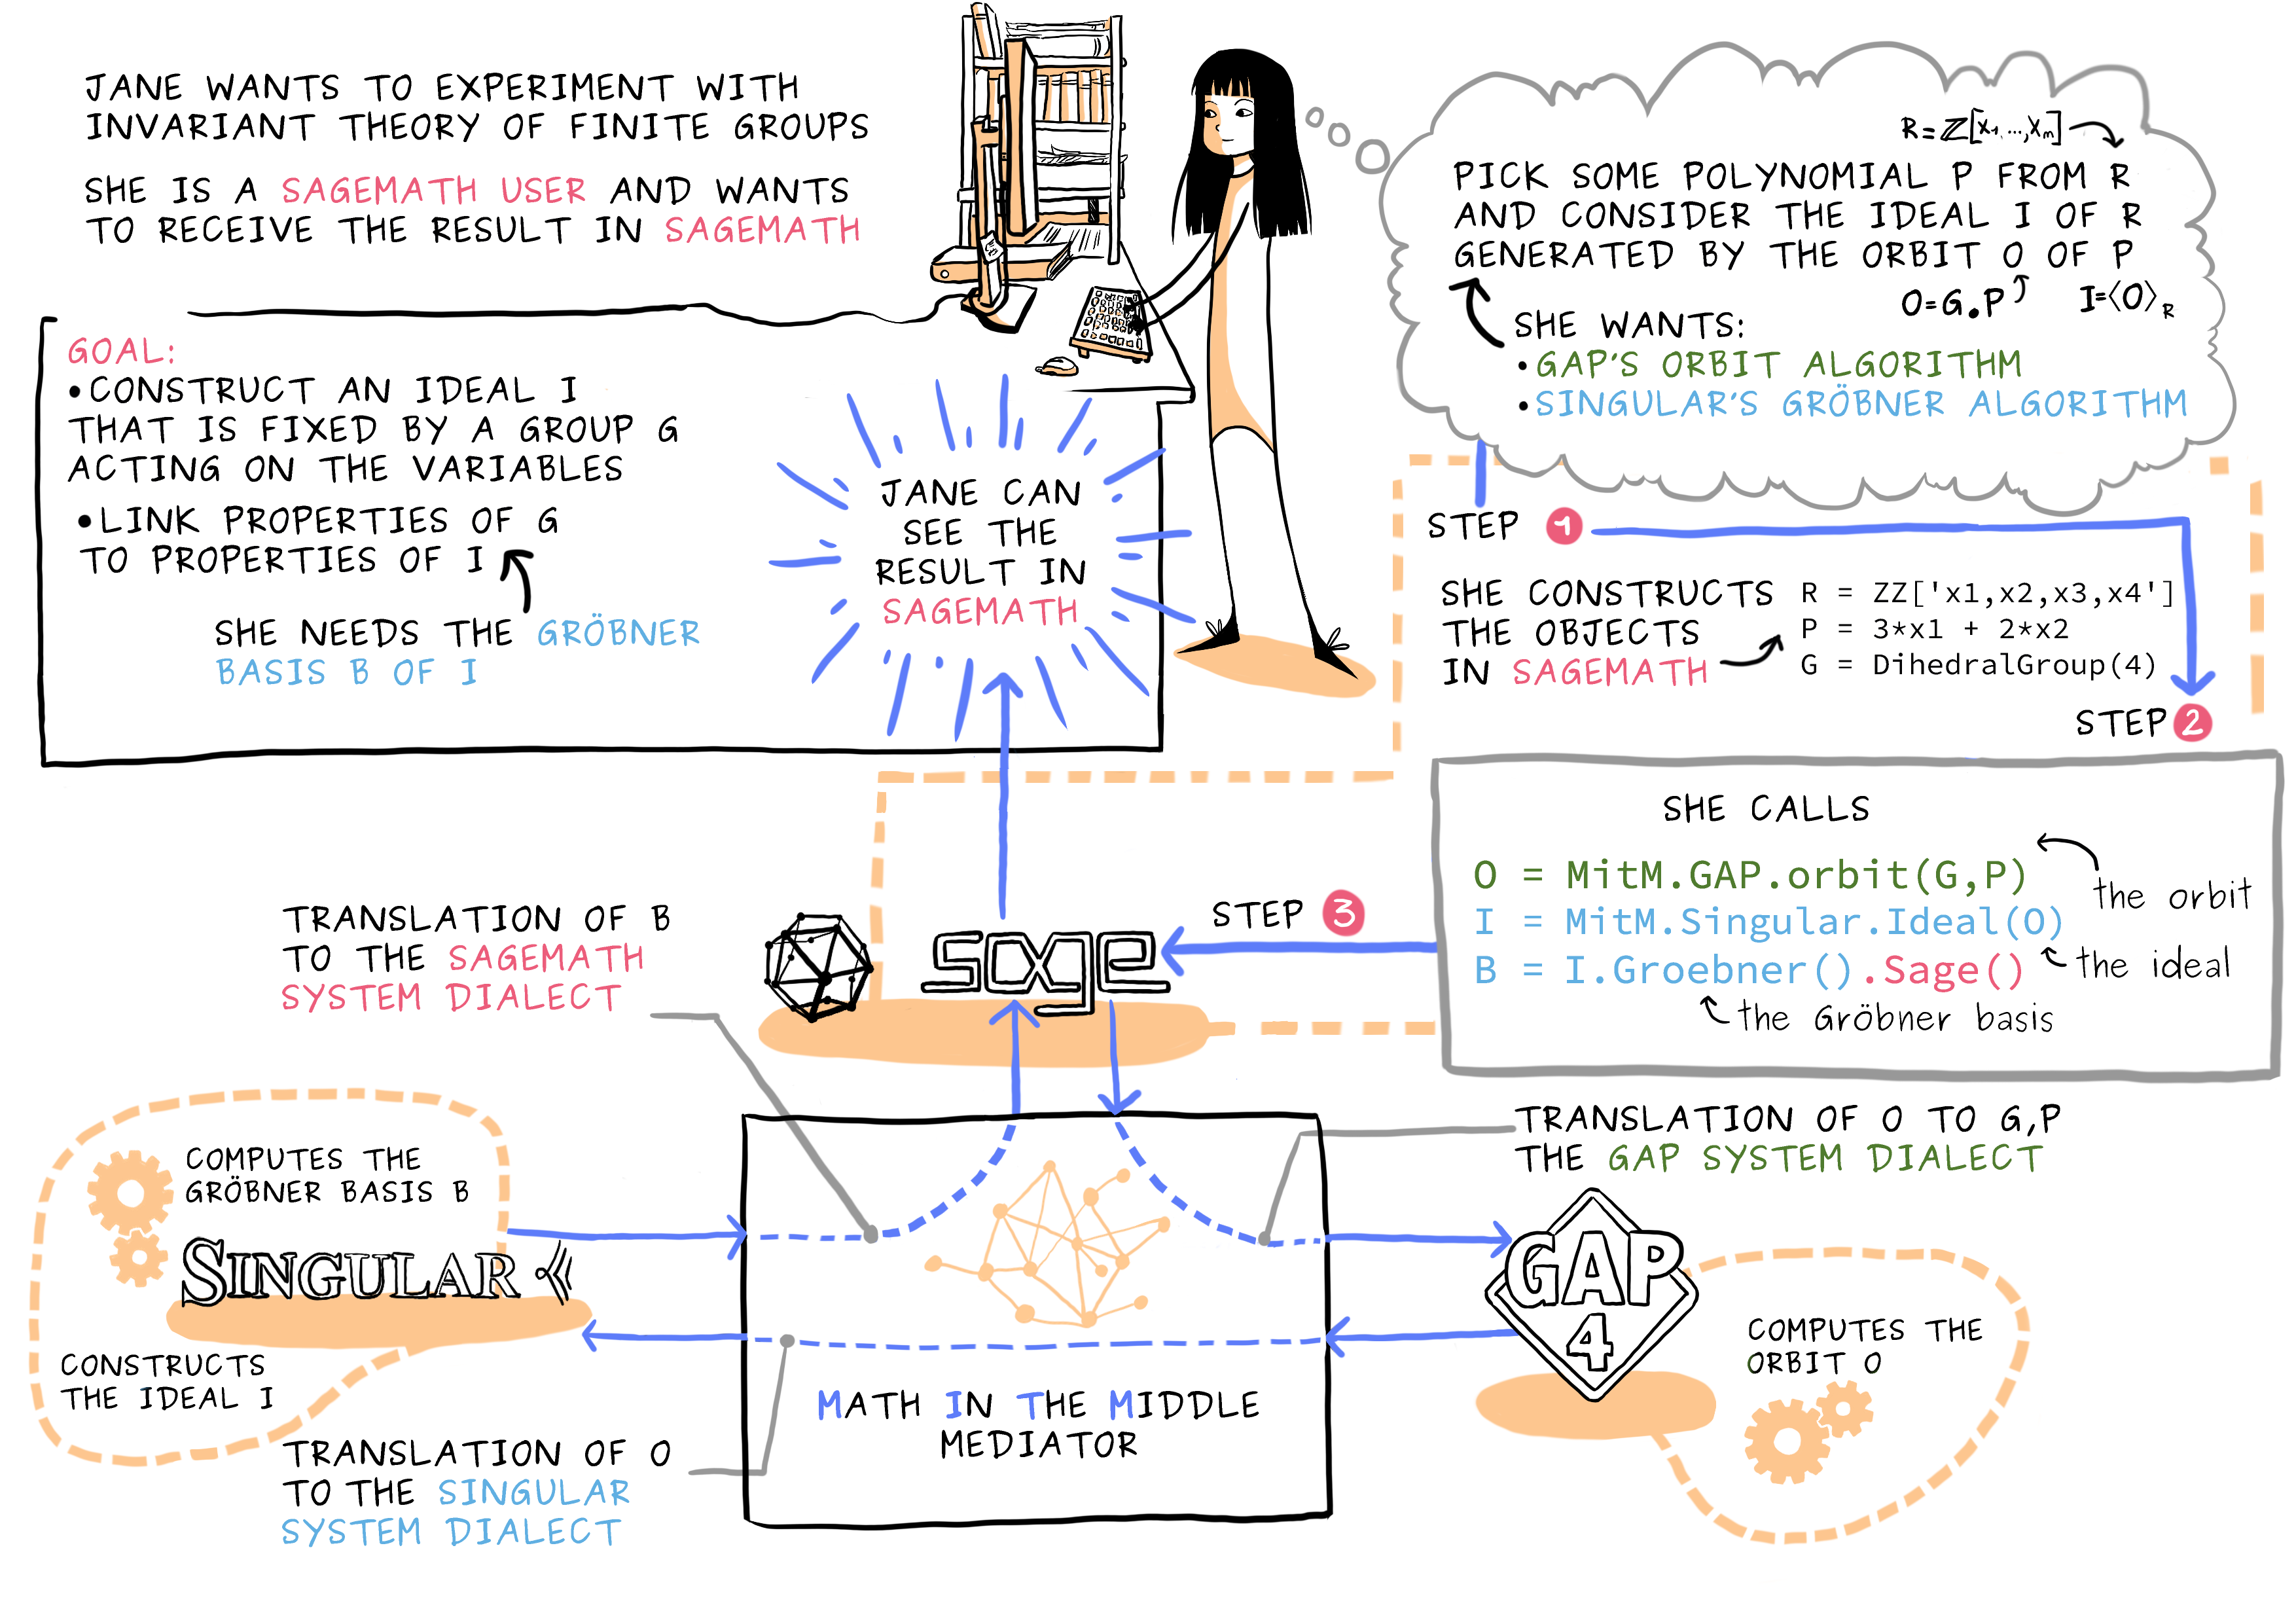
\includegraphics[width=\textwidth]{MitM.png}
\end{frame}

\begin{frame}\frametitle{Integrating BOL and BDL}
\begin{blockitems}{OWL-near option}
\item use BDL to define the primitive types of BOL
\item use those as types of BOL properties
\item Curry-typing throughout
\lec{easy: just merge the grammars}
\end{blockitems}

\begin{blockitems}{SQL-near option}
\item use BDL to define the primitive types of BOL
\item also add ADTs
\item Church typing more prominent
\lec{open question: ADTs in addition to or instead of BOL concepts}
\end{blockitems}

We assume the latter for now without spelling out the details.
\end{frame}

\begin{frame}\frametitle{BDL-Mediated Interoperability}
Idea
 \begin{itemize}
 \item define data types in BDL \glec{or similar typed ontology language}
 \item use ADTs
 \item generate corresponding
  \begin{itemize}
  \item class definitions for programming languages PL
   \lec{one class per ADT}
  \item table definitions in SQL
   \lec{one table per ADT}
  \end{itemize}
 \item use codecs to convert automatically when interchanging data between PL and SQL
 \end{itemize}

Open research problem
 \lec{no shiny solution yet that can be presented in lectures}
\end{frame}

\begin{frame}\frametitle{Codecs in ADT Definitions}
\begin{blockitems}{SQL table schema = list of fields where field is}
\item name
\item type \glec{only types of database supported}
\end{blockitems}

\begin{blockitems}{BDL semantic table schema = list of fields where field is}
\item name
\item type $T$ of \emph{type system} \glec{independent of database}
\item codec for $T$ using primitive objects of database as codes
\glec{see research paper \url{https://kwarc.info/people/frabe/Research/WKR_virtual_17.pdf}}
\end{blockitems}

Codec could be chosen automatically, but we want to allow multiple users a choice of codecs for the same type.
\end{frame}

\begin{frame}[fragile]\frametitle{Example}
Ontology based on BDL-ADTs with additional codec information:
\begin{lstlisting}[basicstyle=\footnotesize]
schema Instructor
  name:    string      codec StandardString
  age:     int         codec StandardInt
  courses: list Course codec CommaSeparatedList CourseAsName
schema Course
  name:     string     codec StandardString
  credits:  float      codec StandardFloat
  semester: Semester   codec SemesterAsString
\end{lstlisting}
\medskip

Generated SQL tables:
\begin{lstlisting}[basicstyle=\footnotesize]
CREATE TABLE Instructor
  (name string, age int, courses string)
CREATE TABLE Course
  (name string, credits float, semester string)
\end{lstlisting}
\end{frame}

\begin{frame}\frametitle{Open Problem: Non-Compositionality}
\begin{blockitems}{Sometimes optimal translation is non-compositional}
\item example translate $list$-type in ADT to comma-separated string in DB
\item better break up $list\,B$ fields in type $A$ into separate table with columns for $A$ and $B$
\end{blockitems}

Similar problems
\begin{itemize}
\item a pair type in an ADT could be translated to two separate columns
\item an option type in an ADT could translated to a normal column using SQL's NULL value
\end{itemize}
\end{frame}

\begin{frame}\frametitle{Open Problem: Querying}
\begin{itemize}
\item General setup
 \begin{itemize}
 \item write SQL-style queries using at the BDL level
 \item automatically encode values when writing to database from PL
 \item automatically decode query results when reading from DB
 \end{itemize}
\item But queries using semantic operations cannot always be translated to DB
 \begin{itemize}
  \item operation $IsSummer: Semester \to bool$ in BDL
  \item query \lstinline|SELECT * FROM course WHERE $IsSummer$(semester)|
  \item how to map $IsSummer$ to SQL?
 \end{itemize}
\item Ontology operations need commuting operations on codes
\begin{itemize}
\item given $f: A\to B$ in BDL, codecs $C,D$ for $A$ and $B$
\item SQL function $f'$ commutes with $f$ iff \\
  \[B.decode (f'(C.encode\,a)) = f(a)\]
  for all $a:A$
\end{itemize}
\end{itemize}
\end{frame}

\begin{frame}\frametitle{Exercise 5, part 1}
We build on the implementation of BDL and codecs from Exercise 4 and on the database schemas from Exercise 3.

\begin{enumerate}
 \item Extend the implementation to BDL+ADT (see Slide 101).
 \item Extend 
  \begin{itemize}
  \item codecs and codec operators with identifiers $I\bbc (strings)$
  \item ADT fields with codec expressions $c::=I \bnfalt I(c_1\ldots,c_n)$
  \end{itemize}
  and write a function that maps $c$ to the corresponding codec.
\end{enumerate}
\end{frame}

\begin{frame}\frametitle{Exercise 5, part 2}

\begin{enumerate}
\setcounter{enumi}{2}
 \item Write a function that takes a vocabulary (= a list of ADT definitions with codec expressions) and generates an SQL schema for it.
 Use the type returned by the codec as the database type.
 \item Write a function that takes an element $d$ of an ADT and generates the SQL (or CSV) representation of $d$ with all field values encoded by the corresponding codec.
 \item Write a function that takes an ADT name and a SQL or CSV object and applies decoding to build the corresponding ADT element.
 \item Test this by
 \begin{itemize}
 \item writing some of your univis table schemas as ADTs and some example values as ADT elements,
 \item exchanging these with a database and/or via CSV with fellow students' implementations.
 \end{itemize}
\end{enumerate}
\end{frame}

\part{Querying}

\section{Overview}

\begin{frame}\frametitle{General Ideas}
\begin{itemize}
\item Recall
 \begin{itemize}
 \item syntax = context-free grammar
 \item semantics = translation to another language
 \end{itemize}
\item Example: BOL translated to SQL, SFOL, Scala, English
\item Querying = use semantics to answer questions about syntax
\end{itemize}
\medskip

Note:
\begin{itemize}
\item Not the standard definition of querying
\item Design of a new Tetrapod-level notion of querying
 \glec{ongoing research}
\item Subsumes concepts of different names from the various aspects
\end{itemize}
\end{frame}

\begin{frame}\frametitle{Propositions}
syntax with propositions = \\
designated non-terminals for propositions
\medskip

Examples:
\begin{center}
\footnotesize
\begin{tabular}{l|l}
aspect & basic propositions\\
\hline
ontology language & assertions, concept equality/subsumption\\
programming language & equality for some types\\
database language & equality for base types \\
logic & equality for all types\\
natural language & sentences \\
\end{tabular}
\end{center}

Aspects vary critically in how propositions can be formed
\begin{itemize}
\item any program in computation
\item quantifiers in deductions \glec{undecidable}
\item $IN$ in databases
\end{itemize}
\end{frame}

\begin{frame}\frametitle{Propositions as Queries}
Propositions allow defining queries

\begin{center}
\footnotesize
\begin{tabular}{l|ll}
& Query & Result\\
\hline
deduction & proposition & yes/no \\
concretization & proposition with free variables & true ground instances \\
computation & term & value \\
narration & question & answer \\
\end{tabular}
\end{center}
\end{frame}

\begin{frame}\frametitle{Semantics of Propositions}
syntax with propositions = \\
designated non-terminals for propositions \\
\lec{needed to ask queries}
semantics with theorems = \\
designates some propositions as theorems or contradictions
\lec{needed to answer queries}

Note:
\begin{itemize}
\item A propositions may be neither theorem nor contradiction.
\item We say that language has negation if:\\ $F$ theorem iff $\neg F$ contradiction and vice versa.
\end{itemize}

We write $\vdash F$ if $F$ is theorem.
\end{frame}

\section{Deductive Queries}

\begin{frame}\frametitle{Definition}
We assume
\begin{itemize}
\item a semantics $\sem{-}$ from $l$ to $L$
\item $l$ has propositions
\item there is an operation $\truelift$ that maps translations of $l$-propositions to $L$-propositions
\item $L$ has semantics with propositions
\end{itemize}

We define
\begin{itemize}
\item a deductive query is an $l$-proposition $p$
\item the result is
 \begin{itemize}
 \item yes if $\truelift \sem{p}$ is a theorem of $L$
 \item no if $\truelift \sem{p}$ is a contradiction in $L$
 \end{itemize}
\end{itemize}
\end{frame}

\begin{frame}{Breakout question}
What can go wrong?
\end{frame}

\begin{frame}\frametitle{Problem: Inconsistency}
In general, (in)consistency of semantics
\begin{itemize}
\item Some propositions may be both a theorem and a contradiction.
\item In that case, queries do not have a result.
\end{itemize}

In practice, however:
\begin{itemize}
\item If this holds for some propositions, it typically holds for all of them.
\item In that, we call $L$ inconsistent.
\item We usually assume $L$ to be consistent.
\end{itemize}
\end{frame}


\begin{frame}\frametitle{Problem: Incompleteness}
In general, (in)completeness of semantics
\begin{itemize}
\item We cannot in general assume that every proposition in $L$ is either a theorem or a contradiction.
\item In fact, most propositions are neither.
\item So, queries do not necessarily have a result.
\item We speak of incompleteness. \glec{Note: not the same as the usual (in)completeness of logic}
\end{itemize}

In practice, however:
\begin{itemize}
\item It may be that $L$ is complete for all propositions in the image of $\truelift\sem{-}$.
\item This is the case if $l$ is simple enough \glec{typical for ontology languages}
\end{itemize}
\end{frame}

\begin{frame}\frametitle{Problem: Undecidability}
In general, (un)decidability of semantics:
\begin{itemize}
\item We cannot in general assume that it is decidable whether a proposition in $L$ is a theorem or a contradiction.
\item In fact, it usually isn't.
\item So, we cannot necessarily compute the result of a query.
\item However: If we have completeness, decidability is likely.
 \glec{run provers for $F$ and $\neg F$ in parallel}
\end{itemize}

In practice, however:
\begin{itemize}
\item It may be that $L$ is decidable for all propositions in the image of $\truelift\sem{-}$.
\item This is the case if $l$ is simple enough \glec{typical for ontology languages}
\end{itemize}
\end{frame}

\begin{frame}\frametitle{Problem: Inefficiency}
In general, (in)efficiency of semantics:
\begin{itemize}
\item Answering deductive queries is very slow.
\item Even if we are complete and decidable.
\end{itemize}

In practice, however:
\begin{itemize}
\item Decision procedures for the image of $\truelift\sem{-}$ may be quite efficient.
\item Dedicated implementations for specific fragments.
\item This is the case if $l$ is simple enough \glec{typical for ontology languages}
\end{itemize}
\end{frame}

\section{Contexts and Free Variables}

\begin{frame}\frametitle{Concepts}
Recall the analogy between grammars and typing:

\begin{center}
\begin{tabular}{l|l}
grammars & typing \\
\hline
non-terminal & type \\
production & constructor \\
non-terminal on left of production & return type of constructor \\
non-terminals on right of production & arguments types of constructor \\
terminals on right of production & notation of constructor\\
words derived from non-terminal $N$ & expressions of type $N$
\end{tabular}
\end{center}

We will now add contexts and substitutions.
\end{frame}

\begin{frame}\frametitle{Contexts}
Given a context-free language $l$, we define:

\begin{itemize}
 \item A \emph{context} $\Gamma$ is of the form $x_1:N_1,\ldots,x_n:N_n$ where the
  \begin{itemize}
   \item $x_i$ are names
   \item $N_i$ are non-terminals
  \end{itemize}
  We write this as $\vdash_l \Gamma$.
 \item A \emph{substitution} for $\Gamma$ is of the form $x_1:=w_1,\ldots,x_n:=w_n$ where the
  \begin{itemize}
   \item $x_i$ are as in $\Gamma$
   \item $w_i$ derived from the corresponding $N_i$
  \end{itemize}
  We write this as $\vdash_l \gamma:\Gamma$.
 \item An \emph{expression in context} $\Gamma$ of type $N$ is a word $w$ derived from $N$ using additionally the productions $N_i::= x_i$.\\
 We write this as $\Gamma\vdash_l w:N$.
 \item Given $\Gamma\vdash w:N$ and $\vdash \gamma:\Gamma$ as above, the \emph{substitution of} $\gamma$ in $w$ is obtained by replacing every $x_i$ in $w$ with $w_i$.
 We write this as $w[\gamma]$.
\end{itemize}
\end{frame}


\begin{frame}\frametitle{Contexts under Compositional Translation}
Consider a compositional semantics $\sem{-}$ from $l$ to $L$ between context-free languages.

\begin{itemize}
 \item Every $\vdash_l w:N$ is translated to some $\vdash_L \sem{w}:N'$ for some $N'$.
 \item Compositionality ensures that $N'$ is the same for all $w$ derived from $N$.
 \item We write $\sem{N}$ for that $N'$.
 \item Then we have 
  \[\vdash_l w:N \tb\mimplies\tb \vdash_L \sem{w}:\sem{N}\]
\end{itemize}

Now we translate contexts, substitutions, and variables as well:
\[\sem{x_1:N_1,\ldots,x_n:N_n}:=x_1:\sem{N_1},\ldots,x_n:\sem{N_n}\]
\[\sem{x_1:=w_1,\ldots,x_n:=w_n}:=x_1:=\sem{w_1},\ldots,x_n:=\sem{w_n}\]
\[\sem{x}:=x\]

Then we have
  \[\Gamma\vdash_l w:N \tb\mimplies\tb \sem{\Gamma}\vdash_L \sem{w}:\sem{N}\]
\end{frame}

\begin{frame}\frametitle{Substitution under Compositional Translation}
From previous slide:
\[\sem{x_1:N_1,\ldots,x_n:N_n}:=x_1:\sem{N_1},\ldots,x_n:\sem{N_n}\]
\[\sem{x_1:=w_1,\ldots,x_n:=w_n}:=x_1:=\sem{w_1},\ldots,x_n:=\sem{w_n}\]
\[\sem{x}:=x\]
\[\Gamma\vdash_l w:N \tb\mimplies\tb \sem{\Gamma}\vdash_L \sem{w}:\sem{N}\]

We can now restate the substitution theorem as follows:
  \[\sem{E[\gamma]}=\sem{E}[\sem{\gamma}]\]
\end{frame}

\section{Concretized Queries}

\begin{frame}\frametitle{Definition}
We assume
\begin{itemize}
\item as for deductive queries
\item semantics must be compositional
\end{itemize}

We define
\begin{itemize}
\item a concretized query is an $l$-proposition $p$ in context $\Gamma$
\item a \emph{single} result is a
 \begin{itemize}
 \item a substitution $\vdash_l \gamma:\Gamma$
 \item such that $\vdash_L \truelift \sem{p[\gamma]}$
 \end{itemize}
\item the \emph{result set} is the set of all results
\end{itemize}
\end{frame}

\begin{frame}\frametitle{Example}
\begin{enumerate}
\item BOL ontology:
\[\mathll{concept\, male,\; concept\, person,\;axiom\, male \sqsubseteq person, \\
  individual\, FlorianRabe,\;assertion\, FlorianRabe\, isa\, male}\]
\item Query $x:individual\vdash_{BOL}x \text{ isa } person$
\item Translation to SFOL: $x:\iota\vdash_{SFOL} person(x)$
\item SFOL calculus yields theorem $\vdash_{SFOL}person(FlorianRabe)$
\item Query result $\sem{\gamma}= x:= FlorianRabe$
\item Back-translating the result to BOL: $\gamma= x:= FlorianRabe$
 \glec{back translation is deceptively simple:}
 \glec{translates SFOL-constant to BOL-individual of same name}
\end{enumerate}
\end{frame}

\begin{frame}{Breakout question}
What can go wrong?
\end{frame}

\begin{frame}\frametitle{Problem: Open World}
In general, semantics uses open world:
\begin{itemize}
\item open world: result contains \emph{all known} results
 \lec{same query might yield more results later}
\item closed world: result set contains \emph{all} results
\end{itemize}
 \glec{always relative to concrete database for $L$}

In practice, however,
\begin{itemize}
\item system explicitly assumes closed world
 \glec{typical for databases}
\item users aware of open world and able to process results correctly
\end{itemize}
\end{frame}

\begin{frame}\frametitle{Problem: Infinity of Results}
In general, there may be infinitely many results:
\begin{itemize}
\item e.g., query for all $x$ such that $\vdash x$,
\end{itemize}

In practice, however,
\begin{itemize}
\item systems pull results from finite database \lec{e.g., SQL, SPARQL}
\item systems enumerate results, require user to explicitly ask for more \lec{e.g., Prolog}
\end{itemize}
\end{frame}

\begin{frame}\frametitle{Problem: Back-Translation of Results}
In general, $\sem{-}$ may be non-trivial to invert
\begin{itemize}
\item easy to obtain $\sem{p}$ in context $\sem{\Gamma}$
  \glec{just apply semantics}
\item possible to find substitutions
\[\vdash_L \delta:\sem{\Gamma} \tb\mwhere\tb \sem{\Gamma}\vdash_L \truelift \sem{p}[\delta]\]
  \glec{easiest case: just look them up in database}
\item but how to translate $\delta$ to $l$-substitutions $\gamma$ with
 \[\vdash_l \gamma:\Gamma \tb\mwhere\tb \sem{\Gamma}\vdash_L \truelift \sem{p[\gamma]}\]
 substitution theorem: pick such that $\sem{\gamma}=\delta$
  \glec{the more $\sem{-}$ does, the harder to invert}
\end{itemize}

In practice, however:
\begin{itemize}
\item often only interested in concrete substitutions
\item translation of concrete data usually identity
\end{itemize}
But: practice restricted to what works even if more is needed
\end{frame}


\section{Computational Queries}

\begin{frame}\frametitle{Definition}
We assume
\begin{itemize}
\item the same as for deductive queries
\item semantics has equality/equivalence $\doteq$
\end{itemize}

We define
\begin{itemize}
\item a computational query is an $l$-expression $e$
\item the result is an $l$-expression $e'$ so that $\vdash_L\sem{e}\doteq\sem{e'}$
\end{itemize}
\lec{intuition: $e'$ is the result of evaluating $e$}

If semantics is compositional, $e$ may contain free variables
\lec{evaluate to themselves}
\end{frame}

\begin{frame}\frametitle{Problem: Back-Translation of Results}
In general, $\sem{-}$ may be non-trivial to invert
\begin{itemize}
\item easy to obtain $E:=\sem{e}$
\item possible to find $E'$ with $\vdash_L E'\doteq E$ by working in the semantics
\item non-obvious how to obtain $e'$ such that $\sem{e'}=E'$
\end{itemize}

In practice, however:
\begin{itemize}
\item evaluation meant to simplify, i.e., only useful if $E'$ very simple
\item simple $E'$ usually in the image of $\sem{-}$
\item typical case: $E'$ is concrete data and $e'=E'$ \lec{called a value}
\end{itemize}
\end{frame}

\begin{frame}\frametitle{Problem: Non-Termination}
In general, computation of $E'$ from $E$ might not terminate
\begin{itemize}
 \item while-loops
 \item recursion
 \item $(\lambda x. x\,x)\,(\lambda x. x\,x)$ with $\beta$-rule
 \item simplification rule $x\cdot y \rewrites y\cdot x$ \glec{similar: distributivity, associativity}
\end{itemize}

In practice, however:
\begin{itemize}
\item image of $\sem{-}$ part of terminating fragment
\end{itemize}
But: if $l$ is Turing-complete or undecidable, general termination not possible
\end{frame}

\begin{frame}\frametitle{Problem: Lack of Confluence}
In general, there may be multiple $E'$ that are simpler than $E$
\begin{itemize}
 \item there may be multiple rules that apply to $E$
 \item e.g., $f(g(x))$
  \begin{itemize}
  \item call-by-value: first simplify $g(x)\rewrites y$, then $f(y)\rewrites z$
  \item call-by-name: first plug $g(x)$ into definition of $f$, then simplify
  \end{itemize}
\item Normal vs. canonical form
 \begin{itemize}
 \item normal: $\vdash_L E\doteq E'$
 \item canonical: normal and $\vdash_L E_1\doteq E_2$ iff $E_1'=E_2'$
  \glec{equivalent expressions have identical evaluation}
  \glec{allows deciding equality}
 \end{itemize}
\end{itemize}

In practice, however:
\begin{itemize}
\item image of $\sem{-}$ part of confluent fragment
\item typical: evaluation to a value is canonical form
 \glec{works for BDL-types but not for, e.g., function types}
\end{itemize}
\end{frame}

\section{Narrative Queries}

\begin{frame}\frametitle{Definition}
We assume
\begin{itemize}
\item semantics into natural language
\end{itemize}

We define
\begin{itemize}
\item a narrative query is an $L$-question about some $l$-expressions
\item the result is the answer to the question
\end{itemize}
\end{frame}

\begin{frame}\frametitle{Problem: Unimplementable}
very expressive = very difficult to implement
\begin{itemize}
\item Natural language understanding
 \begin{itemize}
 \item no implementable syntax of natural language
  \glec{needs restriction to controlled natural language}
 \item specifying semantics hard even when controlled
 \end{itemize}
\item Knowledge base for question answering needed
 \begin{itemize}
 \item very large \glec{must include all common sense}
 \item might be inconsistent \glec{common sense often is}
 \item finding answers still very hard
 \end{itemize}
\end{itemize}
 
In practice, however:
\begin{itemize}
 \item accept unreliability \glec{attach probability measures to answers}
 \item implement special cases \glec{e.g., lookup in databases like Wikidata}
 \item search knowledge base for related statements \glec{Google, Watson}
\end{itemize}
\end{frame}


\section{Syntactic Querying}

\begin{frame}\frametitle{Search}
\begin{itemize}
\item ``search'' not systematically separated from ``querying''
\item often interchangeable
\item querying tends to imply formal languages for queries with well-specified semantics
 \lec{e.g., SQL}
\item search tends to imply less targeted process
 \lec{e.g., Google}
\end{itemize}
\lec{we will not distinguish between the two}
\end{frame}

\begin{frame}\frametitle{Syntactic vs. Semantic Querying}
\begin{blockitems}{Semantic querying}
\item Query results specified by vocabulary $V$ but (usually) not contained in it
\item Query answered using semantics of language
\item Challenge: apply semantics to find results
 \begin{itemize}
 \item deductive query $\vdash f:\prop$ requires theorem prover 
 \item computation query $\vdash e:E$ requires evaluator
 \item concrete query $\Gamma\vdash f:\prop$ requires enumerating all substitutions, running theorem prover/evaluator on all of them
 \end{itemize}
\end{blockitems}
\lec{what we've looked at so far}

\begin{blockitems}{Syntactic querying}
\item Query is an expression $e$
\item Result is set of occurrences of $e$ in $V$
\item Independent of semantics
\item Much easier to realize
\end{blockitems}
\end{frame}

\begin{frame}\frametitle{Challenges for Syntactic Search}
Easier to realize $\to$ scale until new challenges arise
\begin{itemize}
\item large vocabularies
 \begin{itemize}
 \item narrative: all text documents in a domain \glec{e.g., all websites, all math papers}
 \item deductive: large repositories of formalization in proof assistants
  \glec{$10^5$ theorems}
 \item computational: package managers for all programming languages
 \item concrete: all databases in a domain \glec{TBs routine}
 \end{itemize}
\item incremental indexing: reindex only new/changed parts
\item incremental search to handle large result sets \glec{pagination}
\item sophisticated techniques for
 \begin{itemize}
 \item indexing: to allow for fast retrieval
 \item similarity: to select likely results
 \item quality: to rank selected results
\end{itemize}
\item integration of some semantic parts
\end{itemize}
\end{frame}

\begin{frame}\frametitle{Overview}
\begin{itemize}
\item Deduction 
 \begin{itemize}
 \item semantic: theorem proving called search
 \item syntactic: text search
 \end{itemize}
\item Concretization
 \begin{itemize}
 \item semantic: complex query languages (nestable queries)
  \glec{SQL, SPARQL}
 \item syntactic: search by identifier (linked data)
 \end{itemize}
\item Computation
 \begin{itemize}
 \item semantic: interpreters called execution
 \item mixed: IDEs search for occurrences, dependencies
 \item syntactic: search in IDE, package manager
\end{itemize}
\item Narration:
 \begin{itemize}
 \item semantic: very difficult
 \item syntactic: bag of words search
 \end{itemize}
\end{itemize}
\end{frame}


\begin{frame}\frametitle{Abstract Definition: Document}
\textbf{Document} =
\begin{itemize}
\item file or similar resource that contains vocabularies
\item often with comments, metadata
\item different names per aspect
\begin{itemize}
\item deduction: formalization, theory, article
\item computation: source files
\item concretization: database, ontology ABox
\item narrative: document, web site
\end{itemize}
\end{itemize}

\textbf{Library} =
\begin{itemize}
\item collection of documents
\item usually structured into folders, files or similar
\item often grouped by user access \glec{e.g., git repository}
\item vocabularies interrelated within and across libraries
\end{itemize}
\end{frame}

\begin{frame}\frametitle{Abstract Definition: Document Fragment}
\textbf{Fragment} = subdivision of documents into nested semantic units

Examples
\begin{itemize}
\item deductive: theory, section, theorem, definition, proof step, etc.
\item computational: class, function, command, etc.
\item concrete: table, row, cell
\item narrative: section, paragraph, etc.
\end{itemize}

Assign unique \textbf{fragment URI}, e.g., LIB/DOC?FRAG where
\begin{itemize}
\item LIB: base URI of library \lec{e.g., repository URL}
\item DOC: path to document within library \lec{e.g., folder structure, file name}
\item FRAG: id of fragment within document \lec{e.g., class name/method name}
\end{itemize}
\end{frame}

\begin{frame}\frametitle{Abstract Definition: Index(er)}
\textbf{Indexer} consists of
\begin{itemize}
\item data structure $O$ for indexable objects
 \lec{specific to aspect, index design}
 \glec{e.g., words, syntax trees}
\item function that maps library to index \glec{the indexing}
\end{itemize}

\textbf{Index entry} consists of
\begin{itemize}
\item object that occurred in the library
\item URI of the containing fragment
\item information on where in the fragment it was found
\end{itemize}

\textbf{Index} = set of index entries
\end{frame}

\begin{frame}\frametitle{Abstract Definition: Query and Result}
Given
\begin{itemize}
\item indexer $I$ with data structure $O$
\item set of libraries
\item union of their indexes  \lec{computed once, queried often}
\end{itemize}

\textbf{Query} = object $\Gamma \vdash^I q:O$

\textbf{Result} consists of
\begin{itemize}
\item index entry with object $o$
\item substitution for $\Gamma$ such that $q$ matches $o$
 \lec{definition of ``match'' index-specific, e.g., $q[\gamma]=o$}
\end{itemize}

\textbf{Result set} = set of all results in the index
\end{frame}

\begin{frame}\frametitle{Bag of Words Search}
Definition:
\begin{itemize}
\item Index data structure = sequences of words (n-grams) up to a certain length
\item Query = bag of words
 \glec{bag = multiset}
\item Match: (most) words in query occur in same n-gram or n-grams near each other
\end{itemize}

Example implementations
 \begin{itemize}
 \item internet search engines for websites
 \item Elasticsearch: open source engine for custom vocabularies
 \end{itemize}

Mostly used for narrative documents
\begin{itemize}
 \item can treat concrete values as words \glec{e.g., numbers}
 \item could treat other expressions as words \glec{works badly}
\end{itemize}

\end{frame}

\begin{frame}\frametitle{Symbolic Search}
Definition:
\begin{itemize}
\item Index data structure = syntax tree (of any grammar) of expressions $o$ with free/bound variables
\item Query = expression $q$ with free (meta-)variables
\item Match: $q[\gamma]=_\alpha o$, i.e., up to variable renaming
\end{itemize}

Example implementation
 \begin{itemize}
 \item MathWebSearch \lec{see separate slides on MathWebSearch in the repository}
 \end{itemize}

Mostly used for formal documents
\begin{itemize}
 \item deductive
 \item computational
\end{itemize}
\end{frame}

\begin{frame}\frametitle{Knowledge Graph Search}
Definition:
\begin{itemize}
\item Index data structure = assertion forming node/edge in a knowledge graph
\item Index = big knowledge graph $G$
\item Query = knowledge graph $g$ with free variables
\item Match: $g[\gamma]$ is part of $G$
\end{itemize}

Example implementations
 \begin{itemize}
 \item SPARQL engines without consequence closure \glec{i.e., the most common case in practice}
 \item graph databases
 \end{itemize}

Mainly used for ABoxes of untyped ontologies
\end{frame}

\begin{frame}\frametitle{Value Search}
Definition:
\begin{itemize}
\item Index data structure = BDL values $v$
\item Query = BDL expression $q$ with free variables
\item Match: $q[\gamma]=v$
\end{itemize}

Example implementations
 \begin{itemize}
 \item no systematic implementation yet
 \item special cases part of most database systems
 \end{itemize}

Could be used for values occurring in any document
\begin{itemize}
 \item all aspects
 \item may need to decode/encode before putting in index
\end{itemize}
\end{frame}

\begin{frame}\frametitle{Cross-Aspect Occurrences}
Observation
\begin{itemize}
\item libraries are written in one primary aspect
\item indexer focuses on one aspect and kind of object
\item but documents may contain indexable objects of any index
\end{itemize}
\end{frame}

\begin{frame}\frametitle{Cross-Aspect Occurrences: Examples}
\begin{itemize}
\item Any library can contain
\begin{itemize}
 \item metadata on fragments
  \begin{itemize}
  \item relation assertions induce knowledge graph structure between fragments
  \item property assertions contain values narrative, symbolic objects, or values
 \end{itemize}
 \item cross-references to fragments of any other library
 \item narrative comments
\end{itemize}
\item Narrative text may contain symbolic expressions \glec{STEM documents}
\item Database table may have columns containing
 \begin{itemize}
 \item text
 \item encoded BDL values
 \item symbolic expression (often as strings)
 \end{itemize}
\item Symbolic fragments may contain database references
 \glec{e.g., when using database for persistent memoization}
\end{itemize}
\end{frame}

\begin{frame}\frametitle{A New Indexing Design}
recent paper \url{https://kwarc.info/people/frabe/Research/BKR_mdql_20.pdf} \glec{with K. Bercic}

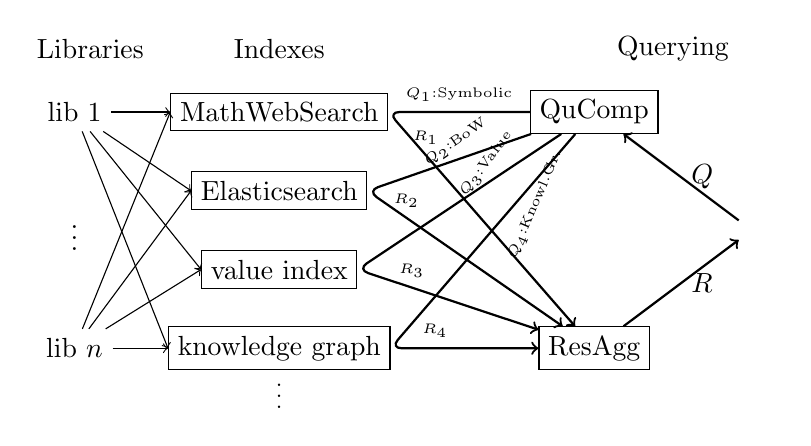
\begin{tikzpicture}[xscale=2]
  \node at (.8,2.8) {Libraries};
  \node (l1) at (0.7,2) {lib 1};
  \node at (.7,.5) {\vdots};
  \node (ln) at (0.7,-1) {lib $n$};
  \node at (2,2.8) {Indexes};
  \node[draw] (si) at (2,2) {MathWebSearch};
  \node[draw] (ni) at (2,1) {Elasticsearch};
  \node[draw] (ci) at (2,0) {value index};
  \node[draw] (oi) at (2,-1) {knowledge graph};
  \node (d) at (2,-1.5]) {\footnotesize\vdots};
  \draw[->] (l1) -- (si);
  \draw[->] (l1) -- (ni.west);
  \draw[->] (l1) -- (oi.west);
  \draw[->] (l1) -- (ci.west);
  \draw[->] (ln) -- (si.west);
  \draw[->] (ln) -- (ni.west);
  \draw[->] (ln) -- (ci.west);
  \draw[->] (ln) -- (oi.west);
  \node at (4.5,2.8) {Querying};
  \node[draw] (qc) at (4,2) {QuComp};
  \node[draw] (qa) at (4,-1) {ResAgg};

  \draw[->,rounded corners,thick] (qc) -- node[above] {\tiny $Q_1$:Symbolic}
                                             (si.east) -- node[pos=.2,above] {\tiny $R_1$} (qa);
  \draw[->,rounded corners,thick] (qc) -- node[pos=.4,above,sloped] {\tiny $Q_2$:BoW}
                                             (ni.east) -- node[pos=.2,above] {\tiny $R_2$} (qa); 
  \draw[->,rounded corners,thick] (qc) -- node[pos=.3,above,sloped] {\tiny $Q_3$:Value}
                                              (ci.east) -- node[pos=.3,above] {\tiny $R_3$} (qa); 
  \draw[->,rounded corners,thick] (qc) -- node[pos=.3,below,sloped] {\tiny $Q_4$:Knowl.Gr.}
                                              (oi.east) -- node[pos=.3,above] {\tiny$R_4$}(qa);

  \node[minimum width=.8cm] (u) at (5,.5) {};

  \draw[->,thick] (u) -- node[right] {$Q$} (qc);
  \draw[->,thick] (qa) -- node[right] {$R$} (u);
\end{tikzpicture}
\end{frame}

\begin{frame}\frametitle{A New Indexing Design (2)}
Tricky question: What is the query language that allows combining queries for each index?
\medskip

Easy:
\begin{itemize}
\item query = conjunction of atomic queries
\item each atom queries one index
\item QuComp splits into atoms
\item ResAgg take intersection of results
\end{itemize}
\medskip

Better: allow variables to be shared across atoms
\lec{open research question}
\end{frame}

\begin{frame}\frametitle{A New Indexing Design: Example}
Consider
\begin{itemize}
\item table of graphs with human-recognizable names and arc-transitivity property\\
indexed into
\begin{itemize}
\item value index for the graph \lec{\texttt{sparse6} codec}
\item Boolean computed property for the arc-transitivity in knowledge graph
\item text index for name
\end{itemize}
\item papers from arXiv in narrative index\\
indexed into
\begin{itemize}
\item narrative index for text
\item MathWebSearch for formulas
\item knowledge graph for metadata
\end{itemize}
\end{itemize}

Query goal: find arc-transitive graphs mentioned by name in articles with h-index greater than 50

%\[\mdql{G:Graph}{\\\cn{arcTransitive}(G), \atomnarr{F}{\cn{Name}(G), \narr{graph}},
% \\\atomorg{F}{\cn{partOf}}{P}, \atomorg{P}{\cn{bibo:publishedIn}}{J}, \atomorg{J}{\cn{spar:hasHindex}}{H}, H > 50}\]
%The first atom in the $\WHERE$-clause returns all arc-transitive graphs $G$ in the concrete index.
%
%The second atom retrieves the names of these graphs and runs a narrative query for them.
%This includes evaluating the expression $\cn{Name}(G)$ into a string by retrieving the corresponding value from the concrete index.
%To avoid false-positives, we include the word $\narr{graph}$ in the narrative atom.
%It instantiates $F$ with the identifier of the matching fragment, presumably a part of a paper.
%
%The next three atoms are organizational atoms that perform a SPARQL query retrieving first the identifier $P$ of the paper containing $F$, the identifiers $J$ of the journal it appeared in, and its h-index $H$.
%$H$ is a concrete value that is reused in the final concrete query on the size of $H$.
%
%Finally, we throw away all variables from the obtained substitutions except for the graphs $G$.
%Alternatively, we could include $P$ in the $\SELECT$-clause to also return the paper.
\end{frame}

\begin{frame}\frametitle{Integrating Semantic Querying}
Word search
\begin{itemize}
\item find multi-meaning words for only one meaning \glec{``normal'' in math}
\item special treatment of certain queries \glec{e.g., ``weather'' in Google}
\end{itemize}

Symbolic search
\begin{itemize}
\item match query $e\doteq e'$ against occurrence $e'\doteq e$
\item similarly: associativity, commutativity, etc.
\item slippery slope to deductive queries
\end{itemize}

Value search
\begin{itemize}
\item match query $1.5$ against interval $1.4\pm 0.2$
\item match query $5\cdot x$ against $25$
\item slippery slope to computational queries
\end{itemize}
\lec{frontiers of research --- in our group: for STEM documents}
\end{frame}

\part{Semantics}

\section{Semantics as Translation}

\begin{frame}\frametitle{Example: Syntax of Arithmetic Language}
Syntax: represented as formal grammar

\begin{commgrammar}
\gcomment{Numbers}\\
\gprod{N}{0\bnfalt 1}{literals}\\
\galtprod{N+N}{sum}\\
\galtprod{N*N}{product}\\
\gcomment{Formulas}\\
\gprod{F}{N\doteq N}{equality}\\
\galtprod{N\leq N}{ordering by size}\\
\end{commgrammar}

Implementation as inductive data type
\end{frame}


\begin{frame}\frametitle{Example: Semantics of Arithmetic Language}
Semantics: represented as translation into known language
\medskip

Problem: Need to choose a known language first\\
Here: unary numbers represented as strings

Built-in data (strings and booleans):
\begin{commgrammar}
%\gcomment{Strings}\\
\gprod{S}{\epsilon}{empty}\\
\galtprod{(\texttt{Unicode)}}{characters}\\
%\gcomment{Booleans}\\
\gprod{B}{\cn{true}}{truth}\\
\galtprod{\cn{false}}{falsity}\\
\end{commgrammar}

Built-in operations to work on the data:
\begin{itemize}
\item concatenation of strings $S\bbc \cn{conc}(S,S)$
\item replacing all occurrences of $c$ in $S_1$ with $S_2$ $S\bbc \cn{replace}(S_1,c,S_2)$
\item equality test: $B\bbc S_1==S_2$
\item prefix test: $B\bbc \cn{startsWith}(S_1,S_2)$
\end{itemize}
\end{frame}

\begin{frame}\frametitle{Example: Semantics of Arithmetic Language}
\begin{blockitems}{Represented as function from syntax to semantics}
\item mutually recursive, inductive functions for each non-terminal symbol
\item compositional: recursive call on immediate subterms of argument
\end{blockitems}

For numbers $n$: semantics $\sem{n}$ is a string
\begin{itemize}
\item $\sem{0}=\epsilon$
\item $\sem{1}="|"$
\item $\sem{m+n}=\cn{conc}(\sem{m},\sem{n})$
\item $\sem{m*n}=\cn{replace}(\sem{m},"|",\sem{n})$
\end{itemize}
\medskip

For formulas $f$: semantics $\sem{f}$ is a boolean
\begin{itemize}
\item $\sem{m\doteq n}=\sem{m}==\sem{n}$
\item $\sem{m\leq n}=\cn{startsWith}(\sem{n},\sem{m})$
\end{itemize}
\end{frame}

\begin{frame}\frametitle{Semantics of BOL}
\begin{center}
\begin{tabular}{lll}
Aspect & kind of semantic language & semantic language\\
\hline 
deduction & logic & SFOL \\
concretization & database language & SQL \\
computation & programming language & Scala \\
narration & natural language & English \\
\end{tabular}
\end{center}

see details of each translation in the lecture notes
\end{frame}

\begin{frame}\frametitle{General Definition}
A semantics by translation consists of
\begin{itemize}
 \item syntax: a formal language $l$
 \item semantic language: a formal language $L$
  \glec{different or same aspect as $l$}
 \item semantic prefix: a theory $P$ in $L$
  \glec{formalizes fundamentals that are needed to represent $l$-objects}
 \item interpretation: translates every $l$-theory $T$ to an $L$-theory $P,\sem{T}$
\end{itemize}
\end{frame}

\begin{frame}\frametitle{Common Principles}
Properties shared by all semantics of BOL
\lec{not part of formal definition, but best practices}
\begin{itemize}
 \item $l$-declaration translated to $L$-declaration for the same name
 \item ontologies translated declaration-wise
 \item one inductive function for every kind of complex $l$-expression
  \begin{itemize}
   \item individuals, concepts, relations, properties, formulas
   \item maps $l$-expressions to $L$-expressions
  \end{itemize}
 \item atomic cases (base cases): $l$-identifier translated to $L$-identifier of the same name
  \glec{or something very similar}
 \item complex cases (step cases): compositional
\end{itemize}
\end{frame}

\begin{frame}\frametitle{Compositionality}
Case for operator $*$ in interpretation function compositional iff \\
interpretation of $*(e_1,\ldots,e_n)$ only depends on on the interpretation of the $e_i$

\[\sem{*(e_1,\ldots,e_n)}=\sem{*}(\sem{e_1},\ldots,\sem{e_n})\]
for some function $\sem{*}$
\bigskip

Example: $;$-operator of BOL in translation to FOL
\begin{itemize}
 \item translation: $\sem{R_1 ; R_2}= \exists m:\iota.\sem{R_1}(x,m)\wedge \sem{R_2}(m,y)$
 \item special case of the above via
  \begin{itemize}
  \item $*=;$
  \item $n=2$
  \item $\sem{;}=(p_1,p_2)\mapsto \exists m:\iota.p_1(x,m)\wedge p_2(m,y)$
  \end{itemize}
 \item Indeed, we have $\sem{R_1;R_2}=\sem{;}(\sem{R_1},\sem{R_2})$
\end{itemize}
\end{frame}


\begin{frame}\frametitle{Compositionality (2)}
Translation compositional iff
\begin{itemize}
\item one translation function for each non-terminal
 \glec{all written $\sem{-}$}
\item each defined by one induction on syntax
 \glec{i.e., one case for production}
 \glec{mutually recursive}
\item all cases compositional
\end{itemize}
\bigskip

Substitution theorem: a compositional translation satisfies
\[\sem{E(e_1,\ldots,e_n)}=\sem{E}(\sem{e_1},\ldots,\sem{e_n})\]
for
\begin{itemize}
\item every expression $E(N_1,\ldots,N_n)$ with non-terminals $N_i$
\item some function $\sem{E}$ that only depends on $E$
\end{itemize}
\end{frame}


\begin{frame}\frametitle{Compositionality (3)}
\[\sem{E(e_1,\ldots,e_n)}=\sem{E}(\sem{e_1},\ldots,\sem{e_n})\]
for every expression $E(N_1,\ldots,N_n)$ with non-terminals $N_i$
\bigskip

Now think of
\begin{itemize}
\item variable $x_i$ of type $N_i$ instead of non-terminal $N_i$
\item $E(x_1,\ldots,x_n)$ as expression with free variables $x_i$ of type $N_i$
\item expressions $e$ derived from $N$ as expressions of type $N$
\item $E(e_1,\ldots,e_n)$ as result of substituting $e_i$ for $x_i$
\item $\sem{E}(x_1,\ldots,x_n)$ as (semantic) expression with free variables $x_i$
\end{itemize}

Then both sides of equations act on $E(x_1,\ldots,x_n)$:
\begin{itemize}
\item left side yields $\sem{E(e_1,\ldots,e_n)}$ by
\begin{itemize}
\item first substitution $e_i$ for $x_i$
\item then semantics $\sem{-}$ of the whole
\end{itemize}
\item right side yields $\sem{E}(\sem{e_1},\ldots,\sem{e_n})$ by
\begin{itemize}
\item first semantics $\sem{-}$ of all parts
\item then substitution $\sem{e_i}$ for $x_i$
\end{itemize}
\end{itemize}
\lec{semantics commutes with substitution}
\end{frame}

\begin{frame}\frametitle{Non-Compositionality}
\begin{blockitems}{Examples}
 \item deduction: cut elimination, translation from natural deduction to Hilbert calculus
 \item computation: optimizing compiler, e.g., loop unrolling
 \item concretization: query optimization, e.g., turning a WHERE of a join into a join of WHEREs,
 \item narration: ambiguous words are translated based on context
\end{blockitems}

\begin{blockitems}{Typical sources}
 \item subcases in a case of translation function
  \begin{itemize}
  \item based on inspecting the arguments, e.g., subinduction
  \item based on context
  \end{itemize}
 \item custom-built semantic prefix
\end{blockitems}
\end{frame}

\section{Context-Sensitive Syntax}

\begin{frame}\frametitle{Definition}
A \textbf{language system} consists of
\begin{itemize}
 \item context-free syntax
 \item distinguished non-terminal symbol $\ThySym$ \glec{words called \textbf{vocabularies}}
 \item some distinguished non-terminal symbols $\ExpSym$ \glec{words called $\ExpSym$-\textbf{expressions}}
 \item unary predicate $\wft{\Theta}$ on vocabularies $\Theta$ \glec{well-formed vocabulary $\Theta$}
 \item unary predicates $\wff{\Theta}{\ExpSym}{E}$ \glec{well-formed $\ExpSym$-expressions $E$}
\end{itemize}
\end{frame}

\begin{frame}\frametitle{Typical Structure}
Vocabularies
\begin{itemize}
\item lists of declarations
\end{itemize}

Declarations
\begin{itemize}
\item named
\item at least one for each expression kind
\item may contain other expressions \glec{e.g., type, definition}
\item may contain nested declarations \glec{e.g., fields in an ADT}
\end{itemize}

Expressions
\begin{itemize}
\item inductive data type
\item relative to vocabulary \glec{names occur as base cases}
\item formulas as special case
\end{itemize}
\end{frame}

\begin{frame}\frametitle{Vocabularies and Expressions}
\begin{center}
\footnotesize
\begin{tabular}{l|ll}
Aspect & vocabulary $\Theta$ & expression kinds $\ExpSym$ \\
\hline
Ontologization  & ontology & individual, concept, relation, property, formula \\
Concretization & database schema & cell, row, table, formula \\
Computation & program & term, type, object, class, \ldots \\
Logic & signature, theory & term, type, formula, \ldots \\
Narration & dictionary & phrases, sentences, texts \\
\end{tabular}
\end{center}
\end{frame}

\begin{frame}\frametitle{Examples}
See notes made during the lecture for examples
\end{frame}

\section{Overview}

\begin{frame}\frametitle{Motivation}
Recall:

\begin{center}
\begin{tabular}{l|l}
Syntax & Data \\
\hline
Semantics & Knowledge
\end{tabular}
\end{center}

Representing
\begin{itemize}
\item syntax = formal language
\begin{itemize}
\item grammar  \glec{context-free part}
\item type system \glec{context-sensitive well-formedness}
\end{itemize}
\item data = words in the syntax
\begin{itemize}
\item set of vocabularies
\item set of typed expressions for each vocabulary
\end{itemize}
\item semantics = \alert{???}
\item knowledge = emergent property of having well-formed words with semantics
\end{itemize}

So far: semantics by translation
\end{frame}

\begin{frame}\frametitle{Relative Semantics}
Semantics by Translation
\begin{itemize}
\item Two syntaxes
\begin{itemize}
\item object-language $l$ \glec{e.g., BOL}
\item meta-language $L$ \glec{e.g., SFOL, Scala, SQL, English}
\end{itemize}
\item Semantics of $L$ assumed fixed
 \glec{captures what we already know}
\item Semantics of $l$ by translation into $L$
\end{itemize}
\lec{semantics of $l$ \emph{relative} to to existing semantics of $L$}

Problem: just kicking the can?
\end{frame}

\begin{frame}\frametitle{Discussion of Relative Semantics}
\begin{blockitems}{Advantages}
\item a few meta-languages yield semantics for many languages
\item easy to develop new languages
\item good connection between syntax and semantics via compositionality, substitution theorem
\end{blockitems}

\begin{blockitems}{Disadvantages}
\item does not solve the problem once and for all
\item impractical without implementation of semantics of meta-language
\item meta-languages typically much more expressive than needed for object-languages
\item translations can be difficult, error-prone
\end{blockitems}

Also needed: absolute semantics
\end{frame}

\begin{frame}\frametitle{Absolute vs. Relative Semantics}
Absolute = self-contained, no use of meta-language $L$

\begin{blockitems}{Get off the ground}
 \item semantics for a few important meta-languages
  \glec{e.g., FOL, assembly language, set theory}
 \item relative semantics for all other languages, e.g.,
  \begin{itemize}
  \item model theory: logic $\to$ set theory
  \item compilation: Scala $\to$ JVM $\to$ assembly
  \end{itemize}
\end{blockitems}

\begin{blockitems}{Redundant semantics}
 \item common to give
 \begin{itemize}
  \item relative and absolute semantics for same syntax
  \item multiple relative semantics
   \glec{translations to different aspects}
  \item sometimes even maybe multiple absolute ones
 \end{itemize}
 \item Allows understanding syntax from multiple perspectives
 \item Allows cross-checking \glec{show equivalence of two semantics}
\end{blockitems}
\end{frame}

\begin{frame}\frametitle{No Perfect Model for Absolute Semantics}
\begin{itemize}
\item Machine-actionable requires reduction to finite set of rules
 \lec{whatever a rule is}
\item Does not work for most domains
 \begin{itemize}
 \item practical argument: any practically interesting system has too many rules
  \glec{cf. physics, e.g., three-body problem already chaotic}
 \item theoretical argument: no language can fully model itself
  \glec{cf. G\"odel's incompleteness theorems}
 \end{itemize}
\item Imperfect representation of intended semantics required
\lec{focus on some \emph{aspect}}
\end{itemize}

Big question: what aspects to focus on?
\end{frame}

\begin{frame}\frametitle{Querying as a Guide}
\begin{blockitems}{Idea}
\item Very difficult to choose aspects for absolute semantics
\item Turn problem around
 \begin{itemize}
 \item ask what the practical purpose of the semantics could be
 \item then choose aspects that allow realizing that purpose
 \end{itemize}
\end{blockitems}

Meta-remark: That's why we did relative semantics and querying first in this course even though absolute semantics conceptually belongs at the beginning.

\begin{blockitems}{Querying as the Purpose}
\item Before: identified different kinds of querying
 \lec{focussing on different aspects of knowledge}
\item Now: each induces a kind of absolute semantics
\end{blockitems}
\end{frame}

%\begin{frame}\frametitle{Problems}
%Next
%\begin{itemize}
%\item four kinds of absolute semantics
% \lec{one per aspect}
%\item Each motivated by one kind of querying
%\item Each defines the aspect
% \glec{e.g., a logic is a language with deductive semantics}
%\end{itemize}
%
%Relation to previous slides
%\begin{itemize}
% \item before: querying via relative semantics
% \item just the special case where target language has corresponding absolute semantics
%  \glec{e.g., deductive querying possible given deductive semantics}
%  \glec{no matter if relative or absolute}
% \item conceptually, absolute semantics comes first, but easier to understand after querying
% \item discussed problems apply to absolute semantics accordingly
%\end{itemize}
%\end{frame}

\section{Absolute Semantics}

\begin{frame}\frametitle{Deductive Semantics}
\begin{blockitems}{Definition}
\item A system that determines which propositions are theorems
 \lec{called a calculus}
\item Languages called logics
\item Implementations called theorem provers
\end{blockitems}

\begin{blockitems}{More precisely}
\item Judgment: $\vdash F$ for ``$F$ is theorem''
\item Set of rules for deriving judgments
\end{blockitems}

\begin{blockitems}{Examples}
\item Natural deduction for first-order logic
\item Axiomatic set theory for (most of) mathematics
\end{blockitems}
\end{frame}

\begin{frame}\frametitle{Redundant Deductive Semantics}
\begin{blockitems}{Multiple deductive semantics}
\item Proof theory: absolute
\item Model theory: relative via translation to set theory $L$
 \glec{write $\models F$ for $\vdash_L \truelift\sem{F}$}
\item Logic translation: relative via translation into standard logics, e.g., SFOL
\end{blockitems}

\begin{blockitems}{Equivalence Theorems}
\item Soundness: $\vdash F$ implies $\models F$
\item Completeness: $\models F$ implies $\vdash F$
\glec{accordingly for other translations}
\end{blockitems}
\end{frame}

\begin{frame}\frametitle{Computational Semantics}
\begin{blockitems}{Definition}
\item A system that evaluates expressions to values
\item Languages typically called programming languages
\item Implementations called interpreters, evaluators
\end{blockitems}

\begin{blockitems}{More precisely}
\item Judgment: $\vdash E\rewrites V$ for ``$E$ evaluates to $V$''
\item Set of rules for deriving $E\rewrites E_1\rewrites E_2\rewrites \ldots$
\item Often more complex judgments using context containing heap, stack, IO channels, local variables
\end{blockitems}

\begin{blockitems}{Examples}
\item Any interpreted language \glec{Python, bash, \ldots}
\item Machine language \glec{interpretation rules built into microchips}
\end{blockitems}
\end{frame}

\begin{frame}\frametitle{Redundant Computation Semantics}
\begin{blockitems}{Multiple computational semantics}
\item Specification: absolute as rules on paper
\item Interpreter: absolute as implementation
\item Compiler: relative via translation to assembly $L$
 \glec{write $\models E\rewrites V$ for $\vdash_L \sem{E}\rewrites \sem{V}$}
\item Cross-compilation: relative via translation into other languages
 \glec{Church-Turing thesis: always possible}
\end{blockitems}

\begin{blockitems}{Equivalence Theorems}
\item Correctness of compiler: $\vdash E\rewrites V$ iff $\models E\rewrites V$
\glec{accordingly for other translations}
\end{blockitems}
\end{frame}

\begin{frame}\frametitle{Concrete Semantics}
\begin{blockitems}{Definition}
\item A system that finds known ground instances of propositions
\item Languages often called query languages
 \glec{inspired our, more general use of the word}
\item Implementations focusing on caching finite sets of ground instances called triple stores, databases
\end{blockitems}


\begin{blockitems}{More precisely}
\item Judgment: $\vdash F[\gamma]$ for ``$\gamma$ is known ground instance of $F$''
\item Set of rules/sets/tables for finding all $\gamma$
\end{blockitems}

\begin{blockitems}{Examples}
\item SQL for Church-typed ontologies with ADTs
\item SPARQL for Curry-typed ontologies
\item Prolog for first-order logic
\end{blockitems}
\end{frame}

\begin{frame}\frametitle{Yes/No vs. Wh-Questions}
Deductive/concrete semantics may be a bit of a misnomer
\begin{itemize}
\item Queries about $\vdash F$ are yes/no questions
 \begin{itemize}
 \item specialty of deductive semantics
 \item but maybe only because everything else is ever harder to do deductively
 \end{itemize}
\item Queries about ground instances of $\Gamma \vdash F$ are Wh questions
 \begin{itemize}
 \item specialty of concrete databases
 \item for the special case of retrieving finite results sets from a fixed concrete store
 \item only situation where Wh questions are easy
 \end{itemize}
\end{itemize}
But Yes/no and Wh questions exist in all aspects.
\end{frame}

\begin{frame}\frametitle{Redundant Concrete Semantics}
\begin{blockitems}{Multiple concrete semantics}
\item Specification: absolute as rules on paper
\item Database: absolute by custom database
\item Database: relative via translation to assembly $L$
\end{blockitems}

\begin{blockitems}{Equivalence Theorems}
\item typically: choose one, no redundancy, no equivalence theorems
\item infinite results: easy on paper, hard in database
\item open world: are all known ground instances in database?
\end{blockitems}
\end{frame}

\begin{frame}\frametitle{Narrative Semantics}
\begin{blockitems}{Definition}
\item Describes how to answer (some) questions
\item Implementations tend to be AI-complete, hypothetical
\item In practice, information retrieval = find related documents
\end{blockitems}

\begin{blockitems}{More precisely?}
\item Not much theory, wide open research problem
\item Some natural language document with interspersed definitions, formulas
\item Maybe judgment: $\vdash Q ? A$ for ``$A$ is answer to $Q$''
\end{blockitems}

\begin{blockitems}{Examples}
\item ``W3C Recommendation OWL 2'' and Google
\item ``ISO/IEC 14882: 1998 Programming Language C++'' and Stroustrup's book
\item Mathematics textbooks and mathematicians
\end{blockitems}
\end{frame}

\section{An Abstract Definition}

\begin{frame}\frametitle{Languages}
\begin{blockitems}{A formal system $l$ consists of}
\item a set of vocabularies $\Voc^l$
\item for every $V\in\Voc^l$, a set $\Exp^l(V)$ of expressions
\item a typing relation $\vdash^l_V e:E$ between $e,E\in \Exp^l(V)$
 \glec{define: $\Exp^l_V(E)=\{e\in \Exp^l_V\,|\,\vdash^l_V e:E\}$}
\end{blockitems}
\glec{convention: leave out superscript $l$, subscript $V$ if clear}

\begin{blockitems}{A formal system with propositions}
\item additionally has a distinguished expression $\prop$
\item define $F$ is proposition if $\vdash_V F:\prop$
\end{blockitems}

\begin{blockitems}{A formal system with equality}
\item additionally has a distinguished proposition $e_1\doteq_E e_2$ whenever $\vdash e_i:E$
\end{blockitems}
\glec{in the sequel: fix $l$ as above}
\end{frame}

\begin{frame}\frametitle{Deductive Semantics}
A deductive semantics for $l$ consists of
\begin{itemize}
\item for every $V$, a subset $\Thm^l_V\sq \Exp^l_V(\prop)$ of theorems
 \glec{write $\vdash^l_V F$ for $F\in\Thm^l_V$}
\end{itemize}
\end{frame}

\begin{frame}\frametitle{Curry-Howard}
Define deductive semantics as a special case of typing
\begin{itemize}
\item propositions as types
\item proofs as expressions
\item add typing rules such that $\vdash P:F$ captures the statement ``$P$ is proof of $F$''
\item define: $\vdash F$ iff there is $P$ such that $\vdash P:F$
\end{itemize}
\end{frame}

\begin{frame}\frametitle{Computational Semantics}
\begin{blockitems}{A computational semantics for $l$ consists of}
\item for every $V$, a function $\Eval^l_V:\Exp^l_V\to\Exp^l_V$
\item the image of $\Eval$ called the values
\glec{write $\vdash^l_V e\rewrites e'$ for $e'=\Eval^l_V(e)$}
\end{blockitems}

\begin{blockitems}{If we also have typing, we say}
 \item subject reduction: if $\vdash e:E$, then $\vdash \Eval(e):E$
\end{blockitems}

\begin{blockitems}{If we also have equality and deductive semantics, we say}
 \item normal forms:
  \begin{itemize}
  \item $\Eval^l_V$ idempotent, i.e., $\Eval^l_V(x)=x$ if $x$ value
  \item $\vdash^l_V e\doteq_E\Eval^l_V(e)$
  \end{itemize} 
 \item canonical forms: $\vdash^l_V e_1\doteq_E e_2$ iff $\Eval^l_V(e_1)=\Eval^l_V(e_2)$
\end{blockitems}
\end{frame}

\begin{frame}\frametitle{Interdefinability}
\begin{blockitems}{Given a computational semantics, define a deductive one:}
\item distinguished expression $\vdash \true:\prop$,
\item $\vdash F$ iff $\Eval(F)=\true$
\lec{implies decidability, so usually only possible for some $F$}
\end{blockitems}

\begin{blockitems}{Given a deductive semantics, define computational one:}
\item $\Eval(e)$ is some $e'$ such that $\vdash e\doteq e'$
\lec{trivially normal, but usually not canonical}
\end{blockitems}

Both kinds of semantics add different value. We usually want both.
\end{frame}

\begin{frame}\frametitle{Why Abstract?}
\begin{blockitems}{Our definitions are abstract}
\item $\Exp$, $\Thm$, $\Eval$ just assumed as sets/functions
\item No requirement how they are constructed
 \begin{itemize}
 \item inductive structure of expressions optional
 \item both absolute and relative semantics are special cases
\end{itemize}
\end{blockitems}

\begin{blockitems}{A more concrete definition might demand}
\item $\Exp_V$ defined by grammar
\item type system defined by
 \begin{itemize}
 \item calculus for $\vdash_V e:E$
 \item alternatively: trivial type system where \\
  all non-terminals $N$ are expressions too \\
  and $\vdash E:N$ iff $E$ derived from $N$
 \end{itemize}
\item $\Thm_V$ defined by calculus for $\vdash_V F$
\item $\Eval_V$ defined by calculus for $\vdash_V e \rewrites e'$
\end{blockitems}
\end{frame}

\begin{frame}\frametitle{Syntax with Contexts}
If we want to talk about contexts, too, we need to expand all of the above.

\begin{blockitems}{Syntax with contexts}
\item contexts: for every $V$, a set $\Cont^l_V$
 \glec{write $\vdash_V \Gamma$}
\item substitutions: for $\Gamma,\Delta\in\Cont_V$, a set $\Subs_V(\Gamma,\Delta)$
 \glec{write $\vdash_V \gamma:\Gamma\to\Delta$}
\end{blockitems}

\begin{blockitems}{Expressions in context}
\item expressions: sets $\Exp_V(\Gamma)$
\item substitution application: functions $\Exp(\gamma):\Exp(\Gamma)\to\Exp(\Delta)$ for $\gamma\in\Subs(\Gamma,\Delta)$
\glec{write $\Exp(\gamma)(e)$ as $e[\gamma]$}
\end{blockitems}

\begin{blockitems}{Typing in context}
\item expressions: sets $\Exp_V(\Gamma,E)$, written as $\Gamma\vdash_V e: E$
\item substitution preserves types: if $\Gamma\vdash e:E$ and $\vdash \gamma:\Gamma\to\Delta$, then $\Delta\vdash e[\gamma]:E[\gamma]$
\end{blockitems}
\end{frame}

\begin{frame}\frametitle{Contexts: General Definition}
We can leave contexts abstract or spell out a concrete definition:
\begin{itemize}
\item contexts $\Gamma$ are of the form \[x_1:E_1,\ldots,x_n:E_n\]
 where $E_i\in\Exp(x_1:E_1,\ldots,x_{i-1}:E_{i-1})$
\item for $\Gamma$ as above, substitutions $\Gamma\to \Delta$ are of the form: \[x_1=e_1,\ldots,x_n=e_n\]
 where $\Delta\vdash e_i: E_i[x_1=e_1,\ldots,x_{i-1}=e_{i-1}]$
\end{itemize}
\medskip

This works uniformly for any formal system.
But most formal systems are a bit more restrictive, e.g., by requiring that all $E_i$ are types.
\end{frame}

\begin{frame}\frametitle{Semantics with Contexts}
\begin{blockitems}{Deductive semantics}
\item define: theorem sets $\Thm_V(\Gamma)$
 \glec{write $F\in\Thm_V(\Gamma)$ as $\Gamma\vdash_V F$}
\item such that theorems are preserved by substitution: \\
 if $\Gamma\vdash_V F$ and $\vdash \gamma:\Gamma\to\Delta$, then $\Delta\vdash_V F[\gamma]$
\end{blockitems}

\begin{blockitems}{Computational semantics}
\item define: evaluation functions $\Eval_V(\Gamma):\Exp_V(\Gamma)\to\Exp_V(\Gamma)$
  \glec{write $e'=\Eval_V(\Gamma)(e)$ as $\Gamma\vdash_V e\rewrites e'$}
\item extend to substitutions: $\Eval_V(\Delta)(\ldots,x=e,\ldots)\;=\;\ldots,x=\Eval_V(\Delta)(e), \ldots$
\item require that evaluation is preserved by substitution $\vdash \gamma:\Gamma\to\Delta$ \\
  $\Eval_V(\Delta)(e[\gamma])=\Eval_V(\Delta)(e)[\Eval_V(\Delta)(\gamma)]$
\glec{substitution theorem for $\Eval$ as a translation from $l$ to itself}
\end{blockitems}
\end{frame}

\begin{frame}\frametitle{Concrete Semantics}
\begin{blockitems}{General definitions for substitutions}
\item write $\cdot$ for empty context/substitution
\item ground expression is expression in empty context
 \glec{also called closed; then opposite is open}
\item ground substitution: $\vdash \gamma:\Gamma\to \es$
 \glec{no free variables after substitution}
\item if we have computational semantics: \\ value substitution is ground substitution where all expressions are values
\item if we have deductive semantics: \\
 true instance of $\Gamma\vdash F:\prop$ is $\gamma$ such that $\vdash F[\gamma]$
\end{blockitems}

\begin{blockitems}{A concrete semantics for $l$ consists of}
\item for every $\Gamma\vdash^l_V F:\prop$, a set $\Inst^l_V(\Gamma,F)$ of ground substitutions
 \glec{write $\Gamma\vdash_V\gamma:F$ for $\gamma\in\Inst_V(\Gamma,F)$}
\end{blockitems}
\end{frame}

\begin{frame}\frametitle{Interdefinability}
\begin{blockitems}{Given concrete semantics, define a deductive one}
\item for ground $F$, $\Inst(\cdot,F)$ is either $\{\cdot\}$ or $\{\}$
\item $\vdash F$ iff $\Inst(\cdot, F)=\{\cdot\}$
\lec{but concrete semantics usually cannot find all substitutions for all $F$}
\end{blockitems}

\begin{blockitems}{Given concrete semantics, define a computational one}
\item $\vdash e\rewrites e'$ iff $(x=e')\in\Inst(x:E, e\doteq_E x)$
\lec{but concrete semantics usually cannot find that substitution for all $e$}
\end{blockitems}

\begin{blockitems}{Given deductive semantics, define a concrete one}
\item $\Inst(\Gamma,F)=\{\vdash \gamma:\Gamma\to\cdot \;|\;\vdash F[\gamma]\}$
\lec{but deductive semantics usually does not allow computing that set}
\end{blockitems}

\begin{blockitems}{Given computational semantics, define a concrete one}
\item $\Inst(\Gamma,F)=\{\Eval(\cdot,\gamma) \;|\;\vdash \gamma:\Gamma\to\cdot, \;\vdash F[\gamma]\rewrites \true\}$
\item allows restricting results to value substitutions
\lec{composition of previous inter-definitions, inherits both problems}
\end{blockitems}
\end{frame}


\begin{frame}\frametitle{Translations}
\begin{blockitems}{A translation $T$ from formal system $l$ to formal system $L$ consists of}
\item function $\Voc^T:\Voc^l\to\Voc^L$
\item family of functions $\Exp^T_V:\Exp^l_V\to\Exp^L_{\Voc^T(V)}$
\end{blockitems}

\begin{blockitems}{Desirable properties}
\item Should satisfy type preservation:
\[\vdash^l_V e:E \tb\mimplies\tb \vdash^L_{\Voc^T(V)} \Exp^T_V(e):\Exp^T_V(E)\]
\lec{intuition: what we have, is preserved}
\item Might satisfy conservativity: 
\[\vdash^L_{\Voc^T(V)} e':\Exp^T_V(E) \tb\mimplies\tb \vdash^l_V e:E \mforsome e\]
\lec{intuition: nothing new is added}
\end{blockitems}
\end{frame}

\begin{frame}\frametitle{Translation of Contexts}
\begin{blockitems}{Translations extend to contexts and substitutions}
 \item $\Cont^T(\ldots,x:E,\ldots) \;=\;\ldots, x:\Exp^T(E), \ldots$
 \item $\Subs^T(\ldots,x=e,\ldots) \;=\;\ldots, x=\Exp^T(e), \ldots$
 \item $\Exp^T(x)=x$ for all variables
\end{blockitems}

\begin{blockitems}{Desirable properties for arbitrary contexts}
\item Type preservation:
\[\Gamma\vdash^l_V e:E \tb\mimplies\tb \Cont^T_V(\Gamma)\vdash^L_{\Voc^T(V)} \Exp^T_V(e):\Exp^T_V(E)\]
\item Conservativity:
\[\Cont^T_V(\Gamma)\vdash^L_{\Voc^T(V)} e':\Exp^T_V(E) \tb\mimplies\tb \Gamma\vdash^l_V e:E \mforsome e\]
\end{blockitems}
\end{frame}

\begin{frame}\frametitle{Compositionality}
Define: a translation is compositional iff we can show the substitution theorem for it

Given
\[\Gamma\vdash^l_V e:E \tb\vdash^l_V \gamma:\Gamma\to\Delta\]
we have that
\[\Cont^T_V(\Delta)\vdash^L_{\Voc^T(V)}\Exp^T_V(e[\gamma])\doteq_{\Exp^T_V(E[\gamma])}\Exp^T_V(e)[\Subs^T_V(\gamma)] \]

Simplify: write
$T(-)$ for $\Voc^T(-), \Exp_V^T(-)$, $\Cont_V^T(-)$, $\Subs_V^T(-)$
\[T(\Delta)\vdash^L_{T(V)}T(e[\gamma])\doteq_{T(E[\gamma])}T(e)[T(\gamma)] \]
\end{frame}

\begin{frame}\frametitle{Relative Semantics}
Given
 \begin{itemize}
 \item formal systems $l$ and $L$
 \item semantics for $L$
 \item translation $T$ from $l$ to $L$
 \end{itemize}
define semantics for $l$
\medskip

\begin{itemize}
\item deductive: define
 \[\vdash^l_V F \tb\miff\tb \vdash^L_{\Voc^T(V)} \Exp^T_V(F) \]
\item computational: define
 \[\vdash^l_V e\rewrites e' \tb\miff\tb \vdash^L_{\Voc^T(V)}\Exp^T_V(e)\rewrites \Exp^T_V(e')\]
\glec{both work accordingly with a context $\Gamma$}
\item concrete: define
 \[\Gamma\vdash^l_V \gamma:F \tb\miff\tb \Cont^T_V(\Gamma)\vdash^L_{\Voc^T(V)}\Subs^T_V(\gamma):\Exp^T_V(F)\]
\end{itemize}
\end{frame}

\begin{frame}\frametitle{Equivalence of Semantics}
Two semantics $\vdash^1$ and $\vdash^2$ for $l$ are equivalent if they are equal in the abstract sense.
\begin{itemize}
\item deductive: $\vdash^1 F$ iff $\vdash^2 F$
\item computational: $\vdash^1 e\rewrites e'$ iff $\vdash^2 e\rewrites e'$
\item concrete: $\Gamma\vdash^1 \gamma:F$ iff $\Gamma\vdash^2 \gamma:F$
\end{itemize}

Example for deductive semantics:
\begin{itemize}
\item $\vdash^1$ absolute semantics by calculus \\
 e.g., natural deduction for SFOL
\item $\vdash^2$ relatives semantics by translation
 e.g., $L$ is set theory, $T$ is model theory of SFOL
\item Assume proofs-as-expressions
\item Then:
 \begin{itemize}
 \item type preservation = soundness
 \item conservativity = completeness
 \end{itemize}
\end{itemize}
\end{frame}

\begin{frame}\frametitle{Exercise 6: Relative Deductive Semantics for BOL}
\begin{itemize}
\item Implement a translation from BOL to untyped FOL
 \glec{you can drop properties, types, and values}
 \glec{so that only one type of individuals is needed}
\item Use TPTP syntax for FOL
 \glec{see \url{http://www.tptp.org/}}
\item Translate an example ontology
  \glec{pick any ontology with a non-trivial consequence closure}
\item Use a theorem prover for first-order logic to implement a relative deductive semantics for BOL
  \glec{Vampire and E are standard choices}
  \glec{see also \url{http://www.tptp.org/cgi-bin/SystemOnTPTP}}
\item Test by example whether your semantics yields the correct consequence closure
\end{itemize}
\end{frame}

\begin{frame}\frametitle{Example: Relative Computational Semantics for BOL}
Scala, SQL semantics evaluates
\begin{itemize}
\item concept $c$ to
\begin{itemize}
\item SQL: table of individuals
 \lec{result of running query $\sem{c}$}
\item Scala: hashset of individuals
 \lec{result of running program $\sem{c}$}
\end{itemize}
\item propositions to booleans \lec{accordingly}
\end{itemize}

Technically, results not in image of $\sem{-}$\\
Fix: add productions for all values
\begin{commgrammar}
\gprod{F}{\true\bnfalt \false}{truth values}\\
\gprod{C}{\{I,\ldots,I\}}{finite concepts}
\end{commgrammar}
\end{frame}

\begin{frame}\frametitle{Equivalence with respect to Semantics}
So far: equivalence of \emph{two semantics} wrt \emph{all queries}

Related concept: equivalence of \emph{two queries} wrt \emph{one semantics}
\begin{itemize}
\item $F$, $G$ deductively equivalence: \[\vdash F \tb\miff\tb \vdash G\]
\glec{may be internalized by syntax as proposition $F\equiv G$}
\item $F,G$ concretely equivalent: \[\vdash F[\gamma] \tb\miff\tb \vdash G[\gamma]\] for all ground substitutions $\gamma$
\glec{weaker than $\Gamma\vdash F\equiv G$}
\item closed $e,e'$ computationally equivalent: \[\vdash e\rewrites v \tb\miff\tb \vdash e'\rewrites v\]
\glec{may be internalized by syntax as proposition $e\doteq e'$}
\end{itemize}
\end{frame}

\begin{frame}\frametitle{Equivalence with respect to Semantics (2)}
Interesting variants of computational semantics
\begin{itemize}
\item open $e,e'$ extensionally equivalent:
  \[\vdash e[\gamma]\rewrites v \tb\miff\tb \vdash e'[\gamma]\rewrites v\]
  for all ground substitutions $\gamma$
 \lec{equal inputs produce equal outputs}
 \glec{weaker then $\Gamma\vdash e\doteq e'$ --- intensional equivalence}
\item machines $M,M'$ observationally equivalent: \\
  produce equal sequences of outputs for the same sequence of inputs
  \glec{e.g., automata, objects in OO-programming}
\end{itemize}

\lec{choice of semantics defines legal optimizations in compiler}
\end{frame}

\section{Absolute Semantics for BOL}

\begin{frame}\frametitle{Judgments}
Typing:  \[\Gamma\vdash^{BOL}_V e:E\]
Deduction: \[\Gamma\vdash^{BOL}_V F\]

Propositions $\prop$:
\begin{itemize}
\item $C\sqsubseteq D$, $C\Equiv D$
\item all three kinds of assertions
\end{itemize}

Notation:
\begin{itemize}
\item We drop the superscript $^{BOL}$ everywhere.
\item We drop the subscript $_V$ unless we need to use $V$.
\item We drop the context $\Gamma$ unless we need to use/change $\Gamma$.
\end{itemize}
\end{frame}

\begin{frame}\frametitle{Typing}
Trivial intrinsic typing (Church) $\vdash e:^{int} E$
\begin{itemize}
\item $E$ is a non-terminal
\item $e$ an expression derived from $E$
\end{itemize}
\medskip

Refined by extrinsic typing (Curry) $\vdash e :^{ext} E$
\begin{itemize}
\item $e$ is an individual, i.e., $\vdash e :^{int} I$
\item $E$ is a concept, i.e., $\vdash E :^{int} C$
 \glec{where $I$ and $C$ are the non-terminals from the grammar}
\item $e$ has concept $E$, i.e., $\vdash e \isa E$
\end{itemize}
\end{frame}

\begin{frame}\frametitle{Propositions as Types}
Say also $\vdash p:f$ for proofs $p$ of proposition $f$
\lec{in particular: $x:f$ in contexts to make local assumptions}
\medskip

Notation:
\[\Gamma,\; f \tb\text{instead of} \tb \Gamma,\;p:f\]
\glec{sufficient if we only state the rules, not build proofs}
\end{frame}

\begin{frame}\frametitle{Lookup Rules}
The main rules that need to access the vocabulary:
\[\rul{f\minn V}{\vdash_V f}\]
\glec{for assertions or axioms f}
\medskip

Assumptions in the context are looked up accordingly:
\[\rul{x:f\minn \Gamma}{\Gamma\vdash f}\]
\end{frame}

\begin{frame}\frametitle{Rules for Subsumption and Equality}
Subsumption is an order with respect to equality:
\[\rul{}{\vdash c\sqsubseteq c}\]

\[\rul{\vdash c\sqsubseteq d \tb \vdash d\sqsubseteq e}{\vdash c\sqsubseteq e}\]

\[\rul{\vdash c\sqsubseteq d \tb \vdash d\sqsubseteq c}{\vdash c\Equiv d}\]

Equal concepts can be substituted for each other:
\[\rul{\vdash c\Equiv d\tb x:C\vdash f(x):\prop \tb \vdash f(c)}{\vdash f(d)}\]

\glec{This completely defines equality.}
\end{frame}

\begin{frame}\frametitle{Rules relating Instancehood and Subsumption}
\[\rul{\vdash i\isa c \tb \vdash c\sqsubseteq d}{\vdash i\isa d}\]
Read:
\begin{itemize}
\item if
 \begin{itemize}
 \item $i\isa c$
 \item $c\sqsubseteq d$
 \end{itemize}
\item then $i\isa d$
\end{itemize}

\[\rul{x:I,\,x\isa c\vdash x\isa d}{\vdash c\sqsubseteq d}\]
Read:
\begin{itemize}
\item if
 \begin{itemize}
 \item assuming an individual $x$ and $x\isa c$, then $x\isa d$
 \end{itemize}
\item then $c\sqsubseteq d$
\end{itemize}
\end{frame}

\begin{frame}\frametitle{Induction}
Consider from before
\[\rul{x:I,\,x\isa c\vdash x\isa d}{\vdash c\sqsubseteq d}\]

Question: Do we allow proving the hypothesis by checking for each individual $x$?
 \lec{induction}
\begin{itemize}
\item<2-> Open world: no
\item<3-> Closed world: yes
 \[\rul{\Gamma[x=i]\vdash f[x=i] \;\text{ for every individual } i}{\Gamma, x:I\vdash f(x)}\]
 \glec{effectively applicable if only finitely many individuals}
\end{itemize}
\end{frame}

\begin{frame}\frametitle{Rules for Union and Intersection of Concepts}
Union as the least upper bound:
\[\rul{}{\vdash c\sqsubseteq c\sqcup d} \tb\tb \rul{}{\vdash d\sqsubseteq c\sqcup d }\]
\[\rul{\vdash c\sqsubseteq h \tb \vdash d\sqsubseteq h}{\vdash c\sqcup d \sqsubseteq h}\]
\medskip

Dually, intersection as the greatest lower bound:
\[\rul{}{\vdash c\sqcap d\sqsubseteq c} \tb\tb \rul{}{\vdash c\sqcap d\sqsubseteq d}\]
\[\rul{\vdash h\sqsubseteq c \tb \vdash h\sqsubseteq d}{\vdash h \sqsubseteq c\sqcap d}\]
\end{frame}

\begin{frame}\frametitle{Rules for Existential and Universal}
Easy rules:
\begin{itemize}
\item Existential
\[\rul{\vdash i\,r\,j \tb \vdash j\isa c}{\vdash i \isa \exists r.c }\]
\item Universal
\[\rul{\vdash i \isa \forall r.c \tb \vdash i\,r\,j}{\vdash j\isa c}\]
\end{itemize}

Other directions are trickier:

\begin{itemize}
\item Existential
\[\rul{\vdash i \isa \exists r.c \tb j:I,\;i\,r\,j,\;j\isa c\vdash f}{\vdash f}\]
\item Universal
\[\rul{j:I,\; i\,r\,j\vdash j\isa c}{\vdash i\isa\forall r.c}\]
\end{itemize}
\end{frame}

\begin{frame}\frametitle{Selected Rules for Relations}
Inverse:
\[\rul{\vdash i \,r\,j}{\vdash j\,r^{-1}\,i}\]

Composition:
\[\rul{\vdash i \,r\,j \tb \vdash j\,s\,k}{\vdash i\,(r;s)\,k}\]

Transitive closure:
\[\rul{}{\vdash i \,r^*\,i} \tb \rul{\vdash i\,r\,j \tb \vdash j\,r^* k}{\vdash i\,r^* k}\]

Identity at concept $c$:
\[\rul{\vdash i \isa c}{\vdash i\,\Delta_c i}\]
\end{frame}

\section{Equivalence of BOL Semantics}

\begin{frame}\frametitle{Overview}
Now $5$ semantics for BOL
\begin{itemize}
\item absolute deductive via calculus
\item relative deductive via SFOL
\item relative computational via Scala
\item relative concrete via SQL
\item relative narrative via English
\end{itemize}
Moreover, these are interdefinable.
\glec{e.g., Scala translation also induces deductive semantics}

Can compare equivalence
\begin{itemize}
\item for every pair of semantics
\item for every kind of equivalence (deductive, concrete, computational)
\end{itemize}
Question: Which of them hold?
\end{frame}

\begin{frame}\frametitle{Questions}
For example, consider:
\begin{itemize}
\item Are the absolute semantics and the Scala semantics deductively equivalent?
\item Assuming BOL and SQL have the base types and values:
Are the absolute semantics and the SQL semantics concretely equivalent?
\end{itemize}
\end{frame}

\begin{frame}\frametitle{Deductive Semantics}
Are these two BOL semantics deductively equivalent
\begin{itemize}
\item absolute deductive semantics 
\item relative deductive semantics via translation $\sem{-}$ to SFOL
\end{itemize}

\only<1>{
Soundness: $\vdash^{BOL}_V f$ implies $\vdash^{SFOL}_{\sem{V}}\sem{f}$ \\
 \begin{itemize}
 \item induction on derivations of $\vdash^{BOL}_V f$
 \item one case per rule
    \glec{induction rule from above not sound}
 \item several pages of work but straightforward and relatively easy
 \end{itemize}
}
\only<2>{
Completeness: $\vdash^{BOL}_V f$ implied by $\vdash^{SFOL}_{\sem{V}}\sem{f}$
 \glec{works if we add missing rules}
\begin{itemize}
\item induction on SFOL derivations does not work
 \begin{itemize}
 \item SFOL more expressive than BOL
 \item $\sem{-}$ not surjective
 \end{itemize}
\item instead show that $\sem{-}$ preserves consistency of vocabularies
 \glec{no universal recipe how to do that}
\item then a typical proof uses $V$ extended with $\neg f$
 \begin{itemize}
 \item if $V$ inconsistent, $\vdash_V f$ for all $f$, done
 \item if $V$ consistent and $V+\neg f$ inconsistent, then $\vdash_V f$, done
 \item if $V+\neg f$ consistent, so is $\sem{V+\neg f}$, which contradicts $\vdash^{SFOL}_{\sem{V}}\sem{f}$
 \end{itemize}
\end{itemize}
}
\end{frame}

\begin{frame}\frametitle{Computational Semantics}
Are these two BOL semantics deductively equivalent
\begin{itemize}
\item absolute deductive semantics 
\item relative deductive semantics via translation $\sem{-}$ to Scala
\end{itemize}

\only<1>{
Soundness: $\vdash^{BOL}_V f$ implies $\vdash^{Scala}_{\sem{V}}\sem{f}\rewrites \true$
\begin{itemize}
\item Problem: Absolute semantics performs consequence closure, e.g.,
\begin{itemize}
\item transitivity of $\sqsubseteq$
\item relationship between $\sqsubseteq$ and $\isa$
\end{itemize}
\item Scala semantics does so only if we explicitly implemented it
\glec{we didn't}
\glec{same problem for SQL semantics}
\end{itemize}
}

\only<2>{
Completness: $\vdash^{BOL}_V f$ implied by $\vdash^{Scala}_{\sem{V}}\sem{f}\rewrites \true$
\begin{itemize}
 \item absolute semantics leaves closed world optional
 \item Scala uses closed worlds
  \glec{e.g., used to compute $c\sqsubseteq d$ by checking all individuals} 
 \item complete only if we add induction rule
\end{itemize}
}
\end{frame}

\end{document}

